\chapter{自然中出现的∞-宇宙}\label{ch:cosmoi-found-in-nature}


在本附录中，我们确立自然中出现的\trInfinityCosmos{}的一些具体例子。通常，
这些\trInfinityCosmos{}的对象是由某个特定的非代数模型所实例化的无穷维%
\trCategory，而其间的\trFunctor{}则是该模型的态射。在大多数情形，都有一个为%
高阶范畴文献所知的\trModelStructure{}与之相伴，它为我们提供恰当的诸%
\trIsofibration{}类、诸\trEquivalence{}类与诸\trTrivialFibration{}类。在指明%
何处可寻得某个合适\trModelStructure{}的存在性证明之后，留给我们的唯一工作，%
便是把先前已确立的诸富集转移为在\trSimplicialSet{}上\trQuasiCategory{}的%
Joyal \trModelStructure{}之上的富集。

我们或可称之为「\trQuasiCategory{}富集的\trModelCategory」的一般理论将在%
E.1 节中讨论。特别地，我们证明任何「\trQuasiCategory{}富集的%
\trCategoryOfFibrantObjects」——即附录 C 中的\cref{def:category-of-fibrant-objects}与%
\cref{def:v-model-category}的一个组合——都定义一个\trInfinityCosmos，并描述一个%
有助于产生例子的\trChangeOfBase{}结果。

在 E.2 节中，我们应用这些结果来确立由\trCompleteSegalSpaces、%
\trSegalCategories{}与 $1$-复状\trSimplicialSet{}诸模型所定义的%
$(\infty,1)$-\trCategory{}的\trInfinityCosmos。它们补充了第 1 章中的%
\cref{prop:cosmos-quasi-categories}所给出的\trQuasiCategory{}的%
\trInfinityCosmos。我们还证明：第 10 章中的\eqref{eq:four-model-cosmoi}%
所展示的诸\trChangeOfModel{}\trFunctor{}定义\trCosmologicalBiequivalence。

最后，在 E.3 节中，我们把注意力转向或许可称作\emph{高阶∞-\trCategory}%
（higher ∞-categories）的对象，确立这样一些\trInfinityCosmos：其对象在%
各种模型中是 $(\infty,n)$-\trCategory，甚至是 $(\infty,\infty)$-\trCategory。


\providecommand{\Fun}{\operatorname{Fun}}
\providecommand{\Cat}{\mathcal{C}at}
\providecommand{\sSet}{s\mathcal{S}et}
\providecommand{\QCat}{\mathcal{Q}\mathcal{C}at}
\providecommand{\Disc}{\mathcal{D}\mathrm{isc}}  %
\providecommand{\qcOne}{\mathbf{1}}   %
\providecommand{\qcInt}{\mathbb{I}}   %
\providecommand{\rvWarrow}{\rightsquigarrow}%
\providecommand{\rvFarrow}{\twoheadrightarrow}%

\section{拟范畴富集的模型范畴}\label{sec:quasi-categorically-enriched-model-categories}

许多\trInfinityCosmos{}的例子，都以一个富集于 Joyal \trModelStructure{}之%
\trSimplicialSet{}上的\trModelCategory{}中\trCategoryOfFibrantObjects{}的形态出现%
——至少当一切\trFibrant{}对象皆\trCofibrant{}时如此，而出人意料的是，情形往往%
正是如此。\footnote{这一假设——一切\trFibrant{}对象皆\trCofibrant{}——对%
\trInfinityCategory{}理论的发展并非本质，尽管它确实使各种证明更为简省。事实上，
文献中首个「∞-宇宙」定义并未包含这一要求 \cite{bib110}。}例如，\trQuasiCategory{}的%
\trInfinityCosmos{}本身就以这种方式出现，因为 Joyal \trModelStructure{}是%
\trCartesianClosed{}（见第 1 章中的\cref{dig:joyal-model-structure}）。Joyal
\trModelStructure{}中的\trFibrant{}对象恰是诸\trQuasiCategory，\trFibrant{}对象之间的%
诸\trFibration{}恰是第 1 章中的\cref{def:isofibration}的诸\trIsofibration，而%
\trFibrant{}对象之间的诸\trWeakEquivalence{}恰是第 1 章中的%
\cref{def:equivalences-quasi-categories}的诸\trEquivalence。

\begin{proposition}\label{prop:fibrant-objects-cosmos}
试设 $\mathcal{M}$ 是任意一个富集于 Joyal \trModelStructure{}之上、且其中每个%
\trFibrant{}对象皆\trCofibrant{}的\trModelCategory。于是，\trFibrant{}对象的全子范畴
$\mathcal{M}_{f}$ 继承一个\trInfinityCosmos{}结构，其中诸\trIsofibration{}是%
\trFibrant{}对象之间的诸\trFibration，诸\trEquivalence{}是\trFibrant{}对象之间的诸%
\trWeakEquivalence，而诸\trTrivialFibration{}是\trFibrant{}对象之间的诸%
\trTrivialFibration。
\end{proposition}
\begin{proof}
由于 $\mathcal{M}$ 中的\trFibrant{}对象亦皆\trCofibrant，附录 C 中的%
\cref{lem:v-model-hom-fibrant}蕴含：$\mathcal{M}$ 中\trFibrant{}–\trCofibrant{}对象
之间的单纯富集 hom 都是\trQuasiCategory，我们将其记作 $\Fun(A,B)$。同一结果还蕴含：
对\trFibrant{}对象之间的任何\trFibration{} $f\colon A\rvFarrow B$，诱导映射
$f_{\ast}\colon\Fun(X,A)\rvFarrow\Fun(X,B)$ 是\trQuasiCategory{}的一个\trIsofibration。

由附录 C 中的\cref{exa:model-category-fibrant-objects}，诸\trFibrant{}对象连同其间
的诸\trFibration{}与诸\trWeakEquivalence{}定义了一个\trCategoryOfFibrantObjects
（见附录 C 中的\cref{def:category-of-fibrant-objects}）。特别地，非富集\trCategory
$\mathcal{M}_{f}$ 拥有一个\trTerminal{}对象、小\trProduct、诸\trIsofibration{}的%
\trPullback，以及诸\trIsofibration{}之可数塔的诸\trLimit，而这些\trLimit{}中的每一个
都在 $\mathcal{M}$ 中被创造。由于 $\mathcal{M}$ 容许单纯\trTensor，附录 A 中的%
\cref{prop:tensors-cotensors-conical}蕴含这些 1-范畴性的\trLimit{}都是锥形的，从而
$\mathcal{M}_{f}$ 拥有\cref{def:infinity-cosmos}(i) 的诸\trConicalLimit。诸%
\trIsofibration{}在\cref{def:infinity-cosmos}(ii) 的 1-范畴性\trLimit{}之下的稳定性，
随即也是附录 C 中的\cref{exa:model-category-fibrant-objects}之%
\trCategoryOfFibrantObjects{}结构的一部分，尽管在许多例子中，诸\trIsofibration{}类的
稳定性也可以经由附录 C 中的\cref{lem:right-lifting-closure}来建立。

尚须验证涉及单纯\trCotensor{}的诸公理。由假设，$\mathcal{M}$ 也余张量化于单纯集之上；
又因 $\mathcal{M}$ 是一个富集模型范畴，\trCotensor{}\trBifunctor{}是一个 Quillen 双变量%
\trAdjunction{}的\trRightAdjoint。直接从附录 C 中的%
\cref{def:quillen-two-variable-adjunction}的定义性公理可知：\trFibrant{}对象对与%
\trCofibrant{}对象作\trCotensor{}后封闭；但由于 Joyal \trModelStructure{}中的一切对象
皆\trCofibrant，\trFibrant{}对象对单纯\trCotensor{}封闭。于是 $\mathcal{M}_{f}$ 拥有
\cref{def:infinity-cosmos}(i) 的一切\trLimit。诸\trIsofibration{}的 Leibniz 稳定性则是
附录 C 中的\cref{def:quillen-two-variable-adjunction}的一个特例，这就证明了
$\mathcal{M}_{f}$ 是一个\trInfinityCosmos。

由于一切\trFibrant{}对象皆\trCofibrant，$\Fun(X,-)\colon\mathcal{M}_{f}\to\QCat$ 是
一支右 Quillen \trFunctor{}在\trFibrant{}对象上的作用（见附录 C 中的%
\cref{ex:quillen-bifunctor-component}），于是由附录 C 中的\cref{lem:quillen-preserves-we}，
$\mathcal{M}_{f}$ 中的诸\trWeakEquivalence{}被送到第 1 章中的%
\cref{def:equivalence-trivial-fibration}的诸\trEquivalence。反之，由第 1 章中的%
\cref{lem:equiv-homotopy-equivalences}，\trInfinityCosmos{}中的每个\trEquivalence{}都
容许一个\trHomotopyEquivalence{}结构——后者用 Quillen 会称之为「右同伦」
（right homotopies）的东西来定义。Quillen 证明：\trModelCategory{}中的任何%
\trHomotopyEquivalence{}都必定是一个\trWeakEquivalence{} \cite[\S1.1]{bib93}。
\end{proof}

再者：

\begin{corollary}\label{cor:right-quillen-adjunction-biequivalence}
任何介于诸拟范畴富集的模型范畴之间的、单纯富集的右 Quillen \trAdjunction——其中一切%
\trFibrant{}对象皆\trCofibrant{}——都定义一个\trCosmologicalFunctor，它每当该 Quillen
\trAdjunction{}定义一个 Quillen \trEquivalence{}时必是一个\trCosmologicalBiequivalence。
\end{corollary}
\begin{proof}
一支右 Quillen \trAdjunction{}保持\trFibrant{}对象，于是单纯富集的右 Quillen
\trAdjunction{}在诸\trFibrant{}对象的子范畴之间定义一个\trSimplicialFunctor，满足%
\trCosmologicalFunctor{}的第一条要求。作为一支右 Quillen \trFunctor，它保持%
\trFibrant{}对象之间的诸\trFibration，从而保持\cref{prop:fibrant-objects-cosmos}所
定义的诸\trInfinityCosmos{}中的诸\trIsofibration。最后，由附录 A 中的%
\cref{prop:enriched-adjoints-preserve-weighted-limits}，单纯富集的\trRightAdjoint{}%
同时保持锥形\trLimit{}与加权\trLimit。这就验证了定义\trCosmologicalFunctor{}的全部公理。

现在试考虑一个单纯富集的右 Quillen \trEquivalence{} $U\colon\mathcal{N}\to\mathcal{M}$，
连同其\trLeftAdjoint{} $F$。\trFunctor{} $U$ 在 hom 上的作用，同构于与一个余单位分量作
前复合所定义的映射：
\begin{center}
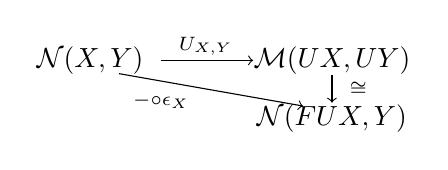
\begin{tikzpicture}[x=1.9em,y=1.5em]
  \node (tl) at (0,1.4) {$\mathcal{N}(X,Y)$};
  \node (tr) at (4.6,1.4) {$\mathcal{M}(UX,UY)$};
  \node (b)  at (4.6,0) {$\mathcal{N}(FUX,Y)$};
  \draw[->] (1.35,1.4) -- (3.1,1.4);
  \node at (2.2,1.74) {$\scriptstyle U_{X,Y}$};
  \draw[->] (0.55,1.08) -- (4.05,0.3);
  \node at (1.35,0.42) {$\scriptstyle -\circ\epsilon_X$};
  \draw[->] (4.6,1.05) -- (4.6,0.38);
  \node at (5.1,0.72) {$\scriptstyle\cong$};
\end{tikzpicture}
\end{center}
其中所示的竖直同构即伴随转置。由附录 C 中的\cref{lem:quillen-equivalence}，余单位分量
$\epsilon_X$ 在 $X$ 是\trFibrant{}的时是一个\trWeakEquivalence。当 $Y$ 是\trFibrant{}的
时，\trFunctor{} $\mathcal{N}(-,Y)\colon\mathcal{N}^{\mathrm{op}}\to\sSet$ 由附录 C 中
的\cref{ex:quillen-bifunctor-component}知是右 Quillen 的。于是，由附录 C 中的%
\cref{lem:quillen-preserves-we}，这一\trFunctor{}把 $\mathcal{N}$ 中\trCofibrant{}对象
之间的诸\trWeakEquivalence{}载为\trQuasiCategory{}之间的诸\trEquivalence。把这些合在一起
便知：当 $X$ 与 $Y$ 是\trFibrant{}的时，对角映射定义\trQuasiCategory{}的一个%
\trEquivalence，从而 $U_{X,Y}\colon\mathcal{N}(X,Y)\to\mathcal{M}(UX,UY)$ 也必定是%
\trQuasiCategory{}的一个\trEquivalence。这就验证了\trCosmologicalBiequivalence{}的%
\trLocalEquivalence{}性质。

本质满性也是附录 C 中的\cref{lem:quillen-equivalence}的一个推论，因为导出单位对任何%
\trFibrant{}对象 $M\in\mathcal{M}$ 都给出一个\trWeakEquivalence{} $M\rvWarrow URFM$。
由于 $RFM$ 是 $\mathcal{N}$ 中的一个\trFibrant{}对象，这就在\trInfinityCosmos{}
$\mathcal{M}_{f}$ 中定义了一个\trEquivalence，涉及 $U\colon\mathcal{N}_{f}\to\mathcal{M}_{f}$
像中的一个对象。
\end{proof}

有了\cref{prop:fibrant-objects-cosmos}，下一个问题便是：富集于 Joyal \trModelStructure{}%
之上的诸\trModelCategory{}从何而来？这一问题在文献中未受多少关注，但在许多情形，相关学界
帮了我们一个大忙：他们提供了由无穷维\trCategory{}组成、却富集于其他某个\trCartesianClosed
\trModelCategory{}之上的诸\trModelCategory。这使我们得以施用附录 C 中的%
\cref{thm:change-of-base-quillen-model}，把一个已知的富集转换为对 Joyal 拟范畴%
\trModelStructure{}的富集。把该结果与\cref{prop:fibrant-objects-cosmos}结合起来，我们便
得到一个有用的\trChangeOfBase{}结果，它产出富集于 Joyal \trModelStructure{}之上的诸%
\trModelCategory。

\begin{proposition}\label{prop:change-of-base-model-cosmoi}
试设 $\mathcal{V}$ 是一个\trCartesianClosed{}模型范畴，它配备一个 Quillen
\trAdjunction，其\trRightAdjoint{}取值于 Joyal \trModelStructure{}，而其\trLeftAdjoint{}%
保持有限\trProduct{}：
\begin{center}
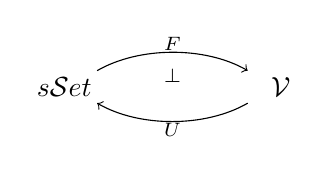
\begin{tikzpicture}[x=1.7em,y=1.4em]
  \node (s) at (0,0) {$\sSet$};
  \node (v) at (4.6,0) {$\mathcal{V}$};
  \draw[->] (0.7,0.42) .. controls (1.6,1.05) and (3.0,1.05) .. (3.9,0.42);
  \node at (2.3,1.12) {$\scriptstyle F$};
  \node at (2.3,0.28) {$\scriptstyle\bot$};
  \draw[->] (3.9,-0.42) .. controls (3.0,-1.05) and (1.6,-1.05) .. (0.7,-0.42);
  \node at (2.3,-1.12) {$\scriptstyle U$};
\end{tikzpicture}
\end{center}
\begin{enumerate}[label=(\roman*)]
\item 则对任何其中每个\trFibrant{}对象皆\trCofibrant{}的 $\mathcal{V}$-模型范畴
  $\mathcal{M}$，\trFibrant{}对象的全子范畴 $\mathcal{M}_{f}$ 定义一个\trInfinityCosmos，
  其中诸\trIsofibration{}是\trFibrant{}对象之间的诸\trFibration，诸\trEquivalence{}是%
  \trFibrant{}对象之间的诸\trWeakEquivalence，诸\trTrivialFibration{}是\trFibrant{}对象
  之间的诸\trTrivialFibration；诸\trFunctorSpace{}由
  $\Fun(M,N)\coloneqq U\mathcal{M}(M,N)$ 定义——其中 $\mathcal{M}(M,N)$ 是 $\mathcal{V}$
  中的 hom-对象；而 $M\in\mathcal{M}_{f}$ 与 $S\in\sSet$ 的单纯\trCotensor{}则由
  $\mathcal{V}$-\trCotensor{} $M^{FS}$ 定义。
\item 此外，任何介于诸此形 $\mathcal{V}$-模型范畴之间的右 Quillen $\mathcal{V}$-伴随都
  定义一个\trCosmologicalFunctor，它每当该 Quillen \trAdjunction{}是一个 Quillen
  \trEquivalence{}时必是一个\trCosmologicalBiequivalence。
\end{enumerate}
\end{proposition}
\begin{proof}
伴随 $F\dashv U$ 被假设为介于诸\trCartesianClosed{}模型范畴之间的一个 Quillen
\trAdjunction，其中\trLeftAdjoint{}保持有限\trProduct。于是，由附录 C 中的%
\cref{thm:change-of-base-quillen-model}，任何 $\mathcal{V}$-模型范畴 $\mathcal{M}$ 都
容有成为一个富集于 Joyal \trModelStructure{}之上的\trModelCategory{}的结构，后者具有
同一个底层非富集模型范畴，其富集 hom 与\trCotensor{}定义为：
\[
\Fun(M,N)\coloneqq U\mathcal{M}(M,N)
\qquad\text{以及}\qquad
M^{S}\coloneqq M^{FS},
\]
如所断言。由于底层模型范畴未曾改变，$\mathcal{M}$ 中的每个\trFibrant{}对象仍是%
\trCofibrant{}的。于是，由\cref{prop:fibrant-objects-cosmos}，\trFibrant{}对象的全子范畴
定义一个\trInfinityCosmos。

再者，由于这一\trChangeOfBase{}结果不影响诸底层模型范畴，任何介于诸 $\mathcal{V}$-模型
范畴之间的右 Quillen 伴随都仍是一支右 Quillen 伴随。由附录 A 中的%
\cref{prop:change-of-base-2-functor}，一个 $\mathcal{V}$-\trFunctor{}在新富集之下成为
单纯富集的\trFunctor。\cref{cor:right-quillen-adjunction-biequivalence}现在告诉我们：
一支右 Quillen $\mathcal{V}$-伴随产生一个\trCosmologicalFunctor，它在那个 Quillen 伴随
是一个 Quillen \trEquivalence{}时是一个\trCosmologicalBiequivalence。
\end{proof}

我们常常在如下特殊情形中利用这一结果：

\begin{corollary}\label{cor:cartesian-closed-cosmos}
试设 $\mathcal{V}$ 是一个其中每个\trFibrant{}对象皆\trCofibrant{}的\trCartesianClosed{}%
模型范畴，它配备一个 Quillen \trAdjunction，其\trRightAdjoint{}取值于 Joyal
\trModelStructure{}，而其\trLeftAdjoint{}保持有限\trProduct{}：
\begin{center}
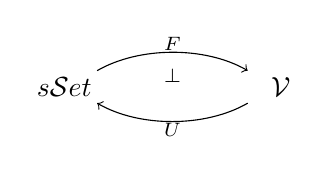
\begin{tikzpicture}[x=1.7em,y=1.4em]
  \node (s) at (0,0) {$\sSet$};
  \node (v) at (4.6,0) {$\mathcal{V}$};
  \draw[->] (0.7,0.42) .. controls (1.6,1.05) and (3.0,1.05) .. (3.9,0.42);
  \node at (2.3,1.12) {$\scriptstyle F$};
  \node at (2.3,0.28) {$\scriptstyle\bot$};
  \draw[->] (3.9,-0.42) .. controls (3.0,-1.05) and (1.6,-1.05) .. (0.7,-0.42);
  \node at (2.3,-1.12) {$\scriptstyle U$};
\end{tikzpicture}
\end{center}
则 $\mathcal{V}$ 的诸\trFibrant{}对象定义一个\trCartesianClosed{}\trInfinityCosmos{}
$\mathcal{V}_{f}$，且其\trRightAdjoint{}定义一个\trCosmologicalFunctor{}
$U\colon\mathcal{V}_{f}\to\QCat$，后者自然同构于底\trQuasiCategory\trFunctor，并每当
$F\dashv U$ 是一个 Quillen \trEquivalence{}时必是一个\trCosmologicalBiequivalence。
\end{corollary}
\begin{proof}
当 $\mathcal{V}$ 的\trFibrant{}对象皆\trCofibrant{}时，$\mathcal{V}$ 本身满足%
\cref{prop:change-of-base-model-cosmoi}(i) 的假设，从而 $\mathcal{V}_{f}$ 定义一个%
\trInfinityCosmos。由附录 A 中的\cref{lem:finite-product-adjunction-v-enriched}，
$F\dashv U$ 在单纯集与单纯富集\trCategory{} $U_{*}\mathcal{V}$ 之间定义一个单纯富集的%
\trAdjunction，这样我们便得到一支单纯富集的右 Quillen \trFunctor{}
$U\colon U_{*}\mathcal{V}\to\sSet$，介于富集于 Joyal \trModelStructure{}之上的诸模型范畴
之间。由\cref{cor:right-quillen-adjunction-biequivalence}，$U$ 进而定义一个%
\trCosmologicalFunctor{} $U\colon\mathcal{V}_{f}\to\QCat$，它在 $F\dashv U$ 是一个
Quillen \trEquivalence{}时是一个\trBiequivalence。把附录 A 中的%
\cref{rem:exponent-one-identity}与\cref{prop:change-of-base-model-cosmoi}所给出的
$\mathcal{V}_{f}$ 之诸\trFunctorSpace{}的定义结合起来，对任何 $X\in\mathcal{V}_{f}$ 我们
便得到下述自然\trIsomorphism
\[
U(X)\cong U(X^{1})\cong\Fun(1,X)
\]
这就证明了\trCosmologicalFunctor{} $U\colon\mathcal{V}_{f}\to\QCat$ 自然同构于配属于%
\trInfinityCosmos{} $\mathcal{V}_{f}$ 的底\trQuasiCategory\trFunctor（另见第 1 章中的%
\cref{rem:underlying-qcat-internal-homs}）。
\end{proof}

\cref{prop:change-of-base-model-cosmoi}启发了如下\trInfinityCosmos{}的平凡例子。

\begin{example}[作为∞-宇宙的 1-范畴]\label{exa:one-categories-as-cosmoi}
任何\trComplete{}且\trLocallySmall $1$-\trCategory{} $\mathcal{E}$ 都可以被造就成一个%
\trInfinityCosmos，其中 $\Fun(A,B)$ 恰是从 $A$ 到 $B$ 的态射之集。由\trYonedaLemma，此时的
诸\trEquivalence{}便是 $\mathcal{E}$ 中的诸\trIsomorphism，于是由第 1 章中的%
\cref{lem:brown-factorization}，一切映射都必定是\trIsofibration。$\mathcal{E}$ 中对象
$A$ 与一个\trSimplicialSet{} $S$ 的\trCotensor{}定义为
\[
A^{S}\coloneqq A^{\pi_{0}S}\coloneqq\prod_{\pi_{0}S}A.
\]
\end{example}

姑且不顾\trModelCategory{}通常被假定除\trLimit{}外还拥有\trColimit{}这一事实，此构造可以
看作\cref{prop:change-of-base-model-cosmoi}施于伴随
\begin{center}
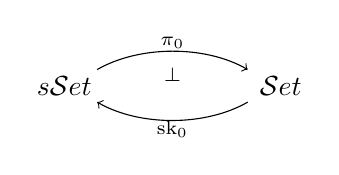
\begin{tikzpicture}[x=1.7em,y=1.4em]
  \node (s) at (0,0) {$\sSet$};
  \node (v) at (4.6,0) {$\mathcal{S}et$};
  \draw[->] (0.7,0.42) .. controls (1.6,1.05) and (3.0,1.05) .. (3.9,0.42);
  \node at (2.3,1.12) {$\scriptstyle\pi_{0}$};
  \node at (2.3,0.28) {$\scriptstyle\bot$};
  \draw[->] (3.9,-0.42) .. controls (3.0,-1.05) and (1.6,-1.05) .. (0.7,-0.42);
  \node at (2.3,-1.12) {$\scriptstyle\mathrm{sk}_{0}$};
\end{tikzpicture}
\end{center}
的一个特例，其\trRightAdjoint{}把 $\mathcal{S}et$ 作为由 0-骨架单纯集构成的子范畴嵌入
$\sSet$（见附录 C 中的\cref{def:simplex-skeleton-coskeleton}）。此处 $\mathcal{S}et$ 上的%
\trCartesianClosed\trModelStructure{}并非附录 C 中的\cref{ex:set-model-category}所考虑的
那一个，而是其中诸\trWeakEquivalence{}为诸\trIsomorphism、一切映射都同时取作余纤维化与
纤维化的那一个。为见这一伴随是 Quillen 的，注意 $\pi_{0}$ 空洞地保持余纤维化，而
$\mathrm{sk}_{0}$ 把任何映射载为\trQuasiCategory{}的一个\trIsofibration：后一断言经由
伴随可得，因为下方左侧的定义性提升性质经转置便给出下方右侧的提升性质：
\begin{center}
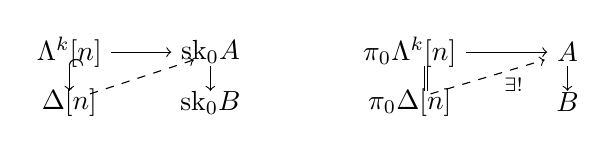
\begin{tikzpicture}[x=1.5em,y=1.4em]
  \node (tl) at (0,1.3) {$\Lambda^k[n]$};
  \node (tr) at (3.4,1.3) {$\mathrm{sk}_{0}A$};
  \node (bl) at (0,0) {$\Delta[n]$};
  \node (br) at (3.4,0) {$\mathrm{sk}_{0}B$};
  \draw[->] (tl) -- (tr);
  \draw[->] (0,0.95) -- (0,0.3);
  \draw (0,0.95) arc[start angle=180,end angle=0,radius=0.16];
  \draw[->,dashed] (0.5,0.22) -- (3.0,1.1);
  \draw[->] (3.4,0.95) -- (3.4,0.3);
  \node at (6.0,0.65) {$\leftrightsquigarrow$};
  \begin{scope}[shift={(8.2,0)}]
    \node (tl2) at (0,1.3) {$\pi_{0}\Lambda^k[n]$};
    \node (tr2) at (3.8,1.3) {$A$};
    \node (bl2) at (0,0) {$\pi_{0}\Delta[n]$};
    \node (br2) at (3.8,0) {$B$};
    \draw[->] (tl2) -- (tr2);
    \draw[double] (0.4,0.95) -- (0.4,0.3);
    \draw[->,dashed] (0.5,0.22) -- (3.25,1.1);
    \node at (2.5,0.45) {$\scriptstyle\exists!$};
    \draw[->] (3.8,0.95) -- (3.8,0.3);
  \end{scope}
\end{tikzpicture}\\[1.2ex]
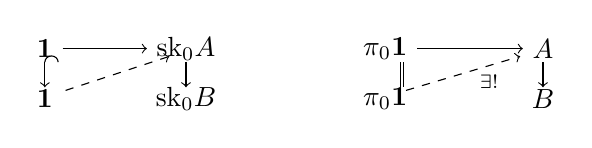
\begin{tikzpicture}[x=1.5em,y=1.4em]
  \node (tl) at (0,1.3) {$\qcOne$};
  \node (tr) at (3.4,1.3) {$\mathrm{sk}_{0}A$};
  \node (bl) at (0,0) {$\qcOne$};
  \node (br) at (3.4,0) {$\mathrm{sk}_{0}B$};
  \draw[->] (tl) -- (tr);
  \draw[->] (0,0.95) -- (0,0.3);
  \draw (0,0.95) arc[start angle=180,end angle=0,radius=0.16];
  \draw[->,dashed] (0.5,0.22) -- (3.0,1.1);
  \draw[->] (3.4,0.95) -- (3.4,0.3);
  \node at (6.0,0.65) {$\leftrightsquigarrow$};
  \begin{scope}[shift={(8.2,0)}]
    \node (tl2) at (0,1.3) {$\pi_{0}\qcOne$};
    \node (tr2) at (3.8,1.3) {$A$};
    \node (bl2) at (0,0) {$\pi_{0}\qcOne$};
    \node (br2) at (3.8,0) {$B$};
    \draw[->] (tl2) -- (tr2);
    \draw[double] (0.4,0.95) -- (0.4,0.3);
    \draw[->,dashed] (0.5,0.22) -- (3.25,1.1);
    \node at (2.5,0.45) {$\scriptstyle\exists!$};
    \draw[->] (3.8,0.95) -- (3.8,0.3);
  \end{scope}
\end{tikzpicture}
\end{center}
众所周知，$\pi_{0}$ 保持有限\trProduct{}，于是\trChangeOfBase{}定理的条件成立。以此方式
产生的\trInfinityCosmos{}之\trHomotopyTwoCategory{}只有恒同 2-\trCell。

\begin{example}[作为∞-宇宙的 2-范畴]\label{exa:two-categories-as-cosmoi}
将上一例范畴化，任何带充分极限的 $2$-\trCategory{} $\mathcal{E}$ 都定义一个%
\trInfinityCosmos，其中 $\Fun(A,B)$ 是 $\mathcal{E}$ 中从 $A$ 到 $B$ 的态射之
hom-\trCategory{}的\trNerve。由第 1 章中的\cref{thm:equivalences-are-equivalences}与
附录 B 中的\cref{prop:equivalences-representably-defined}，诸\trEquivalence{}必定是该
$2$-\trCategory{}中的诸\trEquivalence。受第 1 章中的%
\cref{prop:isofibrations-are-isofibrations}启发，我们取诸\trIsofibration{}为该
$2$-\trCategory{}中的诸\trIsofibration。
\end{example}

若把「充分极限」解作\cref{def:infinity-cosmos}(i) 的诸\trLimit，则剩下的公理%
\cref{def:infinity-cosmos}(ii) 可以手工验证。或者，再一次不顾\trModelCategory{}通常被
假定除\trLimit{}外还拥有\trColimit{}这一事实，我们可以把%
\cref{prop:change-of-base-model-cosmoi}施于第 1 章中的\cref{prop:nerve-left-adjoint}的
同伦范畴$\dashv$\trNerve{}\trAdjunction
\begin{center}
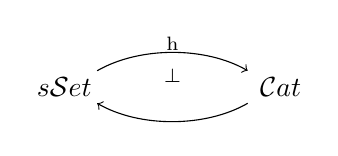
\begin{tikzpicture}[x=1.7em,y=1.4em]
  \node (s) at (0,0) {$\sSet$};
  \node (v) at (4.6,0) {$\Cat$};
  \draw[->] (0.7,0.42) .. controls (1.6,1.05) and (3.0,1.05) .. (3.9,0.42);
  \node at (2.3,1.12) {$\scriptstyle\mathrm{h}$};
  \node at (2.3,0.28) {$\scriptstyle\bot$};
  \draw[->] (3.9,-0.42) .. controls (3.0,-1.05) and (1.6,-1.05) .. (0.7,-0.42);
\end{tikzpicture}
\end{center}
——它是 Joyal \trModelStructure{}与范畴上常见的「民俗」模型结构之间的一个 Quillen
\trAdjunction。任何容有适当有限\trLimit{}与\trColimit{}的 $2$-\trCategory，在配备由
Lack \cite{bib72} 所描述的「平凡」$\Cat$-富集模型结构时，便典范地富集于范畴的民俗模型
结构之上，其弱等价与纤维化恰是刚才描述的那些\trEquivalence{}与\trIsofibration。

尚须揭开「充分极限」这一含糊措辞的含义。由第 6 章中的%
\cref{prop:flexible-weights-homotopical}，$2$-\trCategory{} $\mathcal{E}$ 被要求拥有一切
PIE 极限，即第 6 章中的\cref{dig:flexible-2-limits}所讨论的 2-范畴性的\trProduct、插入子
与均衡化子。据第 6 章中的\cref{def:iso-commas}的构造，这蕴含 $\mathcal{E}$ 容有全部映射
的拟拉回（pseudopullback），但这并不完全蕴含 $\mathcal{E}$ 容有诸\trIsofibration{}的
2-拉回。确切地说，第 6 章中的\cref{lem:iso-commas-pullbacks}之证明构造了一个%
\trIsofibration{}的双拉回（bipullback），其中通常的 hom-\trCategory{}同构被替换为一个
hom-\trCategory{}等价。类似的议论适用于诸\trIsofibration{}之塔的诸\trLimit。但在实践中，
容有 PIE 极限的诸 $2$-\trCategory——例如 \cite{bib18} 所考虑的那些——看来确实容有诸%
\trIsofibration{}的 2-拉回与诸\trIsofibration{}之塔的 2-极限，从而定义出\trInfinityCosmos
的例子。

特别地，把\cref{exa:two-categories-as-cosmoi}特化，便复原出第 1 章中的%
\cref{prop:cosmos-categories}所讨论的 $\Cat$ 上的\trInfinityCosmos{}结构。有趣的是，它也
在 $\Cat^{\mathrm{op}}$ 上定义一个\trInfinityCosmos{}结构，其中的「\trIsofibration」是
那些在对象上单射的\trFunctor。\footnote{在 $\Cat$ 的「民俗」模型结构中，诸纤维化是诸%
\trIsofibration，诸弱等价是诸\trEquivalence，而诸余纤维化是在对象上单射的诸\trFunctor。
在对象上单射的函子满足一个同构扩张性质，它与定义 2-范畴性\trIsofibration{}概念的那个同构
提升性质相对偶。}把这些观察与第 1 章中的\cref{def:co-dual-cosmoi}的对偶∞-宇宙构造结合
起来，便可见四个 2-范畴性的对偶 $\Cat$、$\Cat^{\mathrm{op}}$、$\Cat^{\mathrm{co}}$ 与
$\Cat^{\mathrm{coop}}$ 全都是\trInfinityCosmos。

\cref{exa:two-categories-as-cosmoi}的诸\trInfinityCosmos{}容有一个抽象刻画：它们恰是那些
（作为拟范畴富集的范畴）同构于自身\trHomotopyTwoCategory{}的\trInfinityCosmos。在此情形，
第 3 章中的诸弱 2-极限实际上是严格的，而我们的许多结果都可特化为 2-范畴论文献中已知的定理。

\begin{example}[作为∞-宇宙的单纯模型范畴]\label{exa:simplicial-model-categories-as-cosmoi}
恒同\trFunctor{} $\mathrm{id}\colon\sSet\to\sSet$ 定义一支从 Quillen 的 Kan 复形模型结构
到 Joyal 的拟范畴模型结构的右 Quillen 伴随；显然，其\trLeftAdjoint{}保持\trProduct。于是，
任何 Kan 复形富集的模型范畴——或按惯常的说法，\textbf{单纯模型范畴}
（simplicial model category）——都可以视为一个拟范畴富集的模型范畴，其中\trFibrant{}–%
\trCofibrant{}对象之间的每个\trMappingSpace{}都恰好是一个 Kan 复形。从而，任何\trFibrant{}%
对象皆\trCofibrant{}的单纯模型范畴都可以视为呈现了一个\trInfinityCosmos。
\end{example}

以此方式产生的诸\trHomotopyTwoCategory{}都是 $(2,1)$-\trCategory，其中每个%
\trNaturalTransformation{}都定义一个自然\trIsomorphism。

\begin{digression}[论可达∞-宇宙]\label{dig:accessible-cosmoi}
人们在实践中遇到的许多模型范畴——包括本书考虑的一切例子——都是\emph{组合的}
（combinatorial），意即底范畴是局部可表现的（locally presentable），而模型结构是余纤维性
生成的（cofibrantly generated）。当满足\cref{prop:fibrant-objects-cosmos}之假设的一个
模型范畴 $\mathcal{M}$ 是组合的时，所得的\trInfinityCosmos{} $\mathcal{M}$ 便是一个%
\textbf{可达\trInfinityCosmos}（accessible $\infty$-cosmos）——这是 Bourke 与 Lack 正在研究的
一个概念，它基于他们早先与 Vokřínek 就同伦伴随函子定理所做的合作工作 \cite{bib22}。事实上，
第 6 章中的诸构造很可能都保持可达性，果真如此，则本书考虑的每一座\trInfinityCosmos{}都是
可达的。
\end{digression}

这一观察将有不可胜数的应用留待未来的工作去探究，它们源于把 \cite{bib22} 的主定理特化到这一
情境。首先，任何可达\trInfinityCosmos{}都拥有一切\textbf{柔性加权同伦余极限}，其定义由形如附录 A 中
的\cref{def:weighted-limit-colimit-universal-property}的一个单纯富集泛性质给出，只是以%
\trQuasiCategory{}的\trEquivalence{}而非\trIsomorphism{}来表述。\footnote{\eqref{eq:weighted-universal-property}
中的一切单纯集都是\trQuasiCategory，这一事实是权之柔性的一项推论（见第 6 章中的%
\cref{def:flexible-weights}与\cref{prop:flexible-weights-homotopical}）。}这一结果本身
可以理解为一则第二定理的推论，后者断言：任何介于诸可达\trInfinityCosmos{}之间、作为非富集%
\trFunctor{}为可达的\trCosmologicalFunctor{} $U\colon\mathcal{K}\to\mathcal{L}$ 都容有一个
同伦性的左伴随：对每个 $A\in\mathcal{L}$，都存在 $FA\in\mathcal{K}$ 连同一个映射
$\eta_{A}\colon A\to UFA$，后者对一切 $B\in\mathcal{K}$ 诱导\trQuasiCategory{}的一个%
\trEquivalence
\[
\Fun(FA,B)\rvWarrow \Fun(A,UB)
\]
例如，宇宙论嵌入 $\Disc(\mathcal{K})\hookrightarrow\mathcal{K}$ 恰当 $\mathcal{K}$ 是一个
可达\trInfinityCosmos{}时是可达的，于是这一结果定义了一个弱反射（weak reflection）——它
「自由地逆转」某座\trInfinityCategory{}中的全部箭头。

\subsection*{练习}

\begin{exercise}\label{ex:enriched-fibrant-object-categories}
陈述并证明\cref{prop:change-of-base-model-cosmoi}的一个版本，使之适用于富集的%
\trCategoryOfFibrantObjects——例如\cref{exa:one-categories-as-cosmoi}与%
\cref{exa:two-categories-as-cosmoi}中所考虑的那些——此类范畴可以几乎没有余极限。
\end{exercise}

   %

\providecommand{\Fun}{\operatorname{Fun}}
\providecommand{\Cat}{\mathcal{C}at}
\providecommand{\sSet}{s\mathcal{S}et}
\providecommand{\QCat}{\mathcal{Q}\mathcal{C}at}
\providecommand{\Set}{\mathcal{S}et}
\providecommand{\qcInt}{\mathbb{I}}   %
\providecommand{\CSS}{\mathcal{C}\mathcal{S}\mathcal{S}}
\providecommand{\Segal}{\mathcal{S}egal}
\providecommand{\PCat}{\mathcal{P}\mathcal{C}at}
\providecommand{\OneComp}{1\text{-}\mathcal{C}omp}
\providecommand{\rvDisc}{\mathrm{disc}}
\providecommand{\rvNerve}{\mathrm{nerve}}
\providecommand{\rvLan}{\mathrm{lan}}
\providecommand{\rvRan}{\mathrm{ran}}
\providecommand{\rvDiag}{\mathrm{diag}}

\section{\texorpdfstring{$(\infty,1)$}{(∞,1)}-\trCategory{}的%
\trInfinityCosmos}\label{sec:infinity-cosmoi-of-infinity-1-categories}

\trQuasiCategory{}的\trInfinityCosmos{}已在第 1 章中的%
\cref{prop:cosmos-quasi-categories}中得到确立。在本节中，我们将确立另外三座%
\trInfinityCosmos，其对象定义 $(\infty,1)$-\trCategory——分别以%
\trCompleteSegalSpaces、\trSegalCategories{}或 $1$-复状\trSimplicialSet{}为%
模型——并在它们之间构造下列\trBiequivalence：
\begin{center}
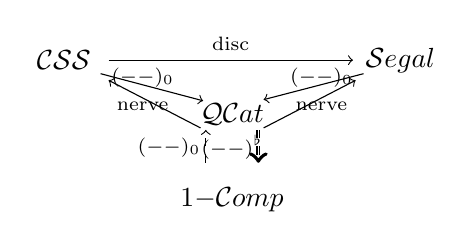
\begin{tikzpicture}[x=1.9em,y=1.4em]
  \node (css)   at (0,2.1)    {$\CSS$};
  \node (segal) at (6.4,2.1)  {$\Segal$};
  \node (qcat)  at (3.2,0.7)  {$\QCat$};
  \node (comp)  at (3.2,-1.5) {$\OneComp$};
  \draw[->] (0.85,2.1) -- node[above]{$\scriptstyle\rvDisc$} (5.5,2.1);
  \draw[->] (0.7,1.75) -- (2.65,1.05);
  \node at (1.5,1.66) {$\scriptstyle(\text{--})_{0}$};
  \draw[->] (2.6,0.35) -- (0.85,1.58);
  \node at (1.5,0.9) {$\scriptstyle\rvNerve$};
  \draw[->] (3.8,0.35) -- (5.55,1.58);
  \node at (4.9,0.9) {$\scriptstyle\rvNerve$};
  \draw[->] (5.7,1.75) -- (3.8,1.08);
  \node at (4.9,1.66) {$\scriptstyle(\text{--})_{0}$};
  \draw[->,dashed] (2.7,-0.55) -- (2.7,0.3);
  \node at (2.0,-0.15) {$\scriptstyle(\text{--})_{0}$};
  \draw[->,dashed,double] (3.7,0.3) -- (3.7,-0.55);
  \node at (3.2,-0.15) {$\scriptstyle(\text{--})^{\flat}$};
\end{tikzpicture}
\end{center}
在给出 Charles Rezk 在 \cite{bib100} 中引入的\trCompleteSegalSpaces{}之形式%
定义之前，我们先解释这一想法。首先，一个\trCompleteSegalSpaces{}是一个%
\textbf{双单纯集}（bisimplicial set）%
$X\in\Set^{\Delta^{\mathrm{op}}\times\Delta^{\mathrm{op}}}$。惯常的做法，是把诸单纯集%
$X_{m\bullet}\coloneqq X_{m,\bullet}$ 视作双单纯集 $X$ 的「列」，而诸单纯集 $X_{\bullet,n}$ 则定义%
「行」。在一个\trCompleteSegalSpaces{}中，如下\trDiagram
\[
X_{\bullet}\coloneqq X_{0}
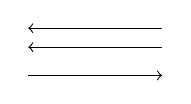
\begin{tikzpicture}[baseline=-0.5ex]
  \draw[<-] (0,0.30) -- (1.7,0.30);
  \draw[<-] (0,0.06) -- (1.7,0.06);
  \draw[->] (0,-0.30) -- (1.7,-0.30);
\end{tikzpicture}
X_{1}
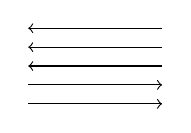
\begin{tikzpicture}[baseline=-0.5ex]
  \draw[<-] (0,0.42) -- (1.7,0.42);
  \draw[<-] (0,0.18) -- (1.7,0.18);
  \draw[<-] (0,-0.06) -- (1.7,-0.06);
  \draw[->] (0,-0.30) -- (1.7,-0.30);
  \draw[->] (0,-0.54) -- (1.7,-0.54);
\end{tikzpicture}
X_{2}\qquad\cdots
\]
定义 Kan 复形的\trCategory{}中的一个\trSimplicialObject。此外，对每个
$m\ge 0$，其余定义域是与该 $m$-\trSimplex{}相伴的「边界数据」之空间的匹配%
映射 $X_{m}\to M_{m}X$ 是一个\trKanFibration。诸空间 $X_{0}$ 与 $X_{1}$ 是%
\trCompleteSegalSpaces{}的「对象与箭头之空间」。所谓的「Segal 条件」蕴含：
空间 $X_{n}$ 可以被视作「$n$-可复合箭头之空间」。一个满足至此所列诸条件的
Segal 空间，便近乎某种「同伦意义上的内范畴」（与附录 B 中的%
\cref{def:internal-category}相比较）。最后一项「完全性」条件把 $X_{0}$ 的
空间性结构与刚刚定义的范畴性结构联系起来，表达了这样一种想法：$X_{0}$ 中的
路径应当对应于 $X_{\bullet}$ 中的诸\trIsomorphism。

\trCompleteSegalSpaces{}的形式定义有三项条件，用\trWeightedLimit{}%
\trBifunctor{}来描述它们最为容易：
\[
(\Set^{\Delta^{\mathrm{op}}})^{\mathrm{op}}\times \sSet^{\Delta^{\mathrm{op}}}
\xrightarrow{\ \operatorname{lim}_{-,-}\ }\sSet
\]
其中 $\sSet$ 被视作一个 $\Set$-富集的\trCategory。注意，$\sSet$ 中
$\Delta^{\mathrm{op}}$-索引之\trDiagram{}的诸权重乃是 $\Set$ 中的
$\Delta^{\mathrm{op}}$-索引之\trDiagram，亦即诸\trSimplicialSet。更为详细地：

\begin{definition}[完全 Segal 空间]\label{def:complete-segal-space}
\begin{enumerate}[label=(\roman*)]
\item 一个\trSimplicialObject{} $X_{\bullet}\in\sSet^{\Delta^{\mathrm{op}}}$
  是\textbf{Reedy 纤维性}的（Reedy fibrant），恰当其在加权极限上诱导的映射
  \[
  X_{m}\cong\operatorname{lim}_{\Delta[m]}X\longrightarrow
  \operatorname{lim}_{\partial\Delta[m]}X=:\ M_{m}X
  \]
  对一切 $m\ge 0$ 都是单纯集之间的\trKanFibration。
\item 一个 Reedy 纤维性的\trSimplicialObject{} $X_{\bullet}$ 是一个%
  \textbf{Segal 空间}（Segal space），恰当其在加权极限上诱导的映射
  \[
  X_{n}\cong\operatorname{lim}_{\Delta[n]}X\longrightarrow
  \operatorname{lim}_{\Lambda^{k}[n]}X
  \]
  对一切 $n\ge 2$ 与 $0<k<n$ 都是单纯集之间的\trTrivialFibration。%
  \footnote{由 Reedy 纤维性，这一诱导映射已经是\trKanFibration，因此要求它
  是\trTrivialFibration，便等价于要求它是一个弱同伦等价。先验地，这一定义
  强于惯常的\textbf{Segal 条件}，后者要求：对每个 $n\ge 2$，由 $n$-%
  \trSimplex{}的\trSpine{}之包含在加权极限上诱导的映射是一个%
  \trTrivialFibration。诸\trSpine{}包含居于由诸内号角包含所胞腔式生成的类
  中，于是把附录 C 中的\cref{ex:leibniz-lifting-equivalences}施于涉及加权
  极限 $\operatorname{lim}$ 的那个双变量伴随，我们的条件显然蕴含经典的
  Segal 条件。其逆向的证明更为精微，可寻于 \cite[3.4]{bib64}。}
\item 一个 Segal 空间 $X_{\bullet}$ 是一个\textbf{\trCompleteSegalSpaces}，
  恰当其在加权极限上诱导的映射
  \[
  \operatorname{lim}_{\qcInt}X\longrightarrow
  \operatorname{lim}_{\Delta[0]}X\cong X_{0}
  \]
  是单纯集之间的一个\trTrivialFibration，此断言谓「$X_{\bullet}$ 中的同构
  之空间」\footnote{别的权重亦可用于定义「同构之空间」，例如%
  $\Delta[2]\xleftarrow{\ \delta^{0}\ }\Delta[1]\xrightarrow{\ \delta^{2}\ }\Delta[2]$ 之\trPushout。关于讨论见 \cite[\S11]{bib100}。}等价于空间
  $X_{0}$。\footnote{由\trTwoOfThreeProperty，这等价于一个可以说更为自然的
  条件：由 $!\colon\qcInt\to\Delta[0]$ 所诱导的映射
  $\Delta\colon X_{0}\to\operatorname{lim}_{\qcInt}X$ 是一个弱同伦等价。}
\end{enumerate}
\end{definition}

双单纯集的\trCategory，作为一个预层范畴，是\trCartesianClosed，从而
富集于其自身之上。在可以把这一富集转换为单纯富集的大量保持乘积的函子
$\Set^{\Delta^{\mathrm{op}}\times\Delta^{\mathrm{op}}}\to\Set^{\Delta^{\mathrm{op}}}$
之中，有两个特别令人感兴趣：$\mathrm{column}_{0}\colon\Set^{\Delta^{\mathrm{op}}\times\Delta^{\mathrm{op}}}\to\Set^{\Delta^{\mathrm{op}}}$，它把双单纯集 $X$
送到其 $0$-单纯形的空间 $X_{0}$；以及 $\mathrm{row}_{0}\colon\Set^{\Delta^{\mathrm{op}}\times\Delta^{\mathrm{op}}}\to\Set^{\Delta^{\mathrm{op}}}$，
它过渡到该\trSimplicialObject{}中每个空间内的顶点之集。正如 Joyal 与
Tierney 所观察到的 \cite{bib64}，前一构造把一个\trCompleteSegalSpaces{}送到
一个\trKanComplex，而后一构造则把一个\trCompleteSegalSpaces{}送到一个%
\trQuasiCategory，它将被用来证明：

\begin{proposition}\label{prop:css-cosmos}
\trCompleteSegalSpaces{}的全子范畴 $\CSS\hookrightarrow\Set^{\Delta^{\mathrm{op}}\times\Delta^{\mathrm{op}}}$ 定义一个\trCartesianClosed{}\trInfinityCosmos，
其中\trFunctorSpace{} $\Fun(A,B)$ 定义为底\trQuasiCategory，它由每个%
\trInternalHom{} $B^{A}$ 中的顶点构成。相对于这一\trInfinityCosmos{}结构：
\begin{enumerate}[label=(\roman*)]
\item 底\trQuasiCategory{}\trFunctor{} $(\text{--})_{0}\coloneqq\mathrm{row}_{0}\colon\CSS\rightleftarrows\QCat$ 是一个%
  \trCosmologicalBiequivalence。
\item 第二个\trCosmologicalBiequivalence{} $\rvNerve\colon\QCat\rightleftarrows\CSS$
  把一个\trQuasiCategory{} $A$ 送到这样一个双单纯集，其 $(m,n)$-单纯形是由%
  \trOrdinalCategory{}与序数\trGroupoid{}之乘积所索引的单纯映射
  $\Delta[m]\times\qcInt[n]\to A$。
\end{enumerate}
\end{proposition}
\begin{proof}
由 Rezk 的一条定理，诸\trCompleteSegalSpaces{}构成承载于双单纯集的%
\trCategory{}之上的一个\trCartesianClosed{}\trModelStructure{}的诸%
\trFibrant{}对象，其中一切对象皆\trCofibrant{} \cite{bib100}。与由
$\pi_{1}([m]\times[n])\coloneqq[m]$ 与 $\iota_{0}([m])\coloneqq[m]\times[0]$
所定义的那对伴随函子作前复合，便诱导出如下方右侧的一个伴随：
\begin{rveq}\label{eq:pi-iota-adjunction}
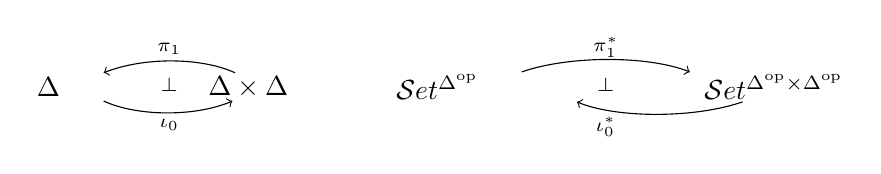
\begin{tikzpicture}[x=1.9em,y=1.5em]
  \node (d)   at (0,0)     {$\Delta$};
  \node (dd)  at (3.8,0)   {$\Delta\times\Delta$};
  \draw[->] (3.55,0.34) .. controls (2.9,0.72) and (1.8,0.72) .. (1.05,0.34);
  \node at (2.3,0.92) {$\scriptstyle\pi_{1}$};
  \node at (2.3,0.05) {$\scriptstyle\bot$};
  \draw[->] (1.05,-0.34) .. controls (1.7,-0.72) and (2.8,-0.72) .. (3.5,-0.34);
  \node at (2.3,-0.92) {$\scriptstyle\iota_{0}$};
  \node at (5.3,0) {$\rightsquigarrow$};
  \node (s)   at (7.4,0)   {$\Set^{\Delta^{\mathrm{op}}}$};
  \node (ss)  at (13.8,0)  {$\Set^{\Delta^{\mathrm{op}}\times\Delta^{\mathrm{op}}}$};
  \draw[->] (9.0,0.36) .. controls (9.9,0.76) and (11.4,0.76) .. (12.2,0.36);
  \node at (10.6,0.96) {$\scriptstyle\pi_{1}^{*}$};
  \node at (10.6,0.05) {$\scriptstyle\bot$};
  \draw[->] (13.2,-0.36) .. controls (12.3,-0.76) and (10.8,-0.76) .. (10.05,-0.36);
  \node at (10.6,-0.96) {$\scriptstyle\iota_{0}^{*}$};
\end{tikzpicture}
\end{rveq}
Joyal 与 Tierney 证明了这一对函子定义拟范畴模型结构与\trCompleteSegalSpaces{}%
模型结构之间的一个 Quillen \trEquivalence{} \cite[4.11]{bib64}。经检视，其%
\trLeftAdjoint{}保持有限\trProduct，于是\cref{cor:cartesian-closed-cosmos}
适用，从而在全子范畴 $\CSS$ 上创造一个\trCartesianClosed{}\trInfinityCosmos{}结构，其细节如\cref{prop:change-of-base-model-cosmoi}所述，
对此 $(\text{--})_{0}\coloneqq\mathrm{row}_{0}=:\ \iota_{0}^{*}$ 是一个%
\trCosmologicalBiequivalence。

第二个介于单纯集与双单纯集之间、方向相反的伴随，其\trLeftAdjoint{}定义为
沿 \trYonedaEmbedding{} $\Delta\times\Delta\hookrightarrow\Set^{\Delta^{\mathrm{op}}\times\Delta^{\mathrm{op}}}$ 对函子
\[
\begin{aligned}
\Delta\times\Delta &\longrightarrow \Set^{\Delta^{\mathrm{op}}}\\
{[m]}\times{[n]} &\longmapsto \Delta[m]\times\qcInt[n]
\end{aligned}
\]
所作的左\trKanExtension；此处 $\qcInt[n]$ 是这样一个\trGroupoid{}的\trNerve：
它恰有 $n+1$ 个对象、且每个 hom-集中恰有一条态射，由自由逆转序数范畴
$\underline{n+1}$ 中的诸态射而得。\trRightAdjoint{}即 (ii) 之陈述中所描述的
那个相应的「$\rvNerve$」函子。Joyal 与 Tierney 还证明了伴随
\begin{center}
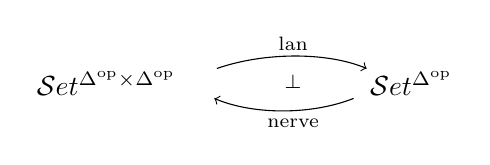
\begin{tikzpicture}[x=1.9em,y=1.5em]
  \node (ss) at (0,0)   {$\Set^{\Delta^{\mathrm{op}}\times\Delta^{\mathrm{op}}}$};
  \node (s)  at (5.8,0) {$\Set^{\Delta^{\mathrm{op}}}$};
  \draw[->] (2.1,0.36) .. controls (3.0,0.76) and (4.2,0.76) .. (4.95,0.36);
  \node at (3.55,0.96) {$\scriptstyle\rvLan$};
  \node at (3.55,0.05) {$\scriptstyle\bot$};
  \draw[->] (4.7,-0.36) .. controls (3.9,-0.76) and (2.8,-0.76) .. (2.05,-0.36);
  \node at (3.55,-0.96) {$\scriptstyle\rvNerve$};
\end{tikzpicture}
\end{center}
相对于\trCompleteSegalSpaces{}与拟范畴的模型结构是一个 Quillen \trEquivalence
\cite[4.12]{bib64}。为了从\cref{cor:right-quillen-adjunction-biequivalence}
得出 $\rvNerve\colon\QCat\to\CSS$ 是一个\trCosmologicalBiequivalence，尚须
证明的只是：这一函子是单纯富集的且保持单纯\trCotensor；或者等价地，由附录 A
中的\cref{prop:enriched-adjoint-preserves-tensors}，伴随
$\rvLan\dashv\rvNerve$ 是单纯富集的。

为验证这一点，我们利用外积\trBifunctor：
\[
\begin{aligned}
\Set^{\Delta^{\mathrm{op}}}\times\Set^{\Delta^{\mathrm{op}}}
&\xrightarrow{\ \square\ }\Set^{\Delta^{\mathrm{op}}\times\Delta^{\mathrm{op}}}\\
(A,\ B) &\longmapsto (A\square B)_{m,n}\coloneqq A_{m}\times B_{n}
\end{aligned}
\]
由于任何双单纯集 $X$ 都可以被复原为诸可表示对象的典范余极限，只需考虑从
可表示双单纯集 $\Delta[m]\square\Delta[n]$ 到单纯集 $A$ 的映射。在刚刚定义
的 $\Set^{\Delta^{\mathrm{op}}\times\Delta^{\mathrm{op}}}$ 之单纯富集中，从
$\Delta[m]\square\Delta[n]$ 到 $\rvNerve(A)$ 的映射单纯集，其 $k$-单纯形定义
为 $\rvNerve(A)^{\Delta[m]\square\Delta[n]}$ 中的 $(k,0)$-单纯形。现在
\[
(\rvNerve(A)^{\Delta[m]\square\Delta[n]})_{k,0}
=\Set^{\Delta^{\mathrm{op}}\times\Delta^{\mathrm{op}}}((\Delta[m]\square\Delta[n])
\times(\Delta[k]\square\Delta[0]),\ \rvNerve(A))
\]
由双单纯集上\trCartesianClosed{}结构的定义而然，而后者
\[
\cong\Set^{\Delta^{\mathrm{op}}\times\Delta^{\mathrm{op}}}((\Delta[m]\times\Delta[k])
\square\Delta[n],\ \rvNerve(A))
\]
由外积的定义而然，后者又
\[
\cong\Set^{\Delta^{\mathrm{op}}}(\rvLan((\Delta[m]\times\Delta[k])\square\Delta[n]),\ A)
\]
由伴随而然。Joyal 与 Tierney 在 \cite[2.11]{bib64} 中证明：左\trKanExtension{}%
作用于外\trTensorProduct{}的方式为 $\rvLan(B\square\Delta[n])\cong B\times\qcInt[n]$。于是我们得到
\[
\begin{aligned}
&\cong\Set^{\Delta^{\mathrm{op}}}((\Delta[m]\times\Delta[k])\times\qcInt[n],\ A)\\
&\cong\Set^{\Delta^{\mathrm{op}}}((\Delta[m]\times\qcInt[n])\times\Delta[k],\ A)\\
&\cong\Set^{\Delta^{\mathrm{op}}}(\rvLan(\Delta[m]\square\Delta[n])\times\Delta[k],\ A)\\
&=:\ (A^{\rvLan(\Delta[m]\square\Delta[n])})_{k}
\end{aligned}
\]
最后一步由单纯集上\trCartesianClosed{}结构的定义而然。这就证明了该伴随与诸
单纯富集相容，于是由\cref{cor:right-quillen-adjunction-biequivalence}与
\cite[4.12]{bib64} 即得：$\rvNerve\colon\QCat\to\CSS$ 是一个%
\trCosmologicalBiequivalence。
\end{proof}

第二种 $(\infty,1)$-\trCategory{}的模型与上述模型密切相关。

\begin{definition}[Segal 范畴]\label{def:segal-categories}
一个\textbf{Segal 前范畴}（Segal precategory）是一个双单纯集
$X_{\bullet}\in\Set^{\Delta^{\mathrm{op}}\times\Delta^{\mathrm{op}}}$，其
$0$-单纯形的空间 $X_{0}$ 在其顶点之集 $X_{0,0}$ 上是 $0$-骨架的。一个%
\textbf{\trSegalCategories{}}是一个 Reedy 纤维性的 Segal 前范畴，%
\footnote{原书此句（A Segal category is a Segal category that is Reedy fibrant and satisfies…）之第二出现疑为「Segal precategory」之误（否则定义
循环），此处径改。——译者注}且满足
\cref{def:complete-segal-space}的 Segal 条件。
\end{definition}

\cref{def:segal-categories}比惯常的定义略强，后者由 Dwyer、Kan 与 Smith
\cite{bib38} 首先引入，又经 Hirschowitz 与 Simpson \cite{bib56} 进一步发展。
惯常的约定定义一个\trSegalCategories{}为一个 Segal 前范畴 $X_{\bullet}$，使
得对每个 $n\ge 2$，由 $n$-\trSimplex{}的\trSpine{}之包含
$\Gamma[n]\hookrightarrow\Delta[n]$ 在加权极限上诱导的映射
\[
X_{n}\cong\operatorname{lim}_{\Delta[n]}X\longrightarrow
X_{1}\times_{X_{0}}\cdots\times_{X_{0}}X_{1}\cong
\operatorname{lim}_{\Gamma[n]}X
\]
\footnote{原书此式末项印作「$\operatorname{lim}_{\Gamma[n]}\Delta[n]$」，疑为
「$\operatorname{lim}_{\Gamma[n]}X$」之误——同式首项作
$\operatorname{lim}_{\Delta[n]}X$，且该映射由 $n$-\trSimplex{}的\trSpine{}之包含
$\Gamma[n]\hookrightarrow\Delta[n]$ 在加权极限上诱导，此处径改。——译者注}
是单纯集之间的一个弱同伦等价——而不要求 Reedy 纤维性。我们更愿意把 Reedy
纤维性纳入我们的\trSegalCategories{}概念之中，使得诸\trSegalCategories{}恰是
Segal 前范畴的\trCategory{} $\PCat$ 上某个适当模型结构中的诸\trFibrant{}对象，
而该模型结构随之产出一个\trInfinityCosmos。在我们引入\trInfinityCosmos{}
$\Segal$ 之前，我们先解释如何把一个\trCompleteSegalSpaces{}变换为一个%
\trSegalCategories。

\begin{lemma}\label{lem:discretization}
存在一个称作\textbf{离散化}（discretization）的函子 $\rvDisc\colon\Set^{\Delta^{\mathrm{op}}\times\Delta^{\mathrm{op}}}\to\Set^{\Delta^{\mathrm{op}}\times\Delta^{\mathrm{op}}}$，由下列\trPullback{}定义%
\footnote{原书本引理中离散化函子之定义域与余定义域两处、以及下文两处%
$\PCat$ 之包含，上标均印作短形 $\Set^{\Delta^{\mathrm{op}}}$；按数学文义
（离散化系双单纯集的自函子，$\PCat$ 系双单纯集之子范畴）均应为%
$\Set^{\Delta^{\mathrm{op}}\times\Delta^{\mathrm{op}}}$，径改。——译者注}
\begin{center}
\begin{tikzpicture}[x=2.1em,y=1.5em]
  \node (dl) at (0,1.5)   {$\rvDisc(X)$};
  \node (tr) at (5.4,1.5) {$X$};
  \node (bl) at (0,0)     {$\mathrm{cosk}_{0}(X_{0,0})$};
  \node (br) at (5.4,0)   {$\mathrm{cosk}_{0}(X_{0})$};
  \draw[right hook->] (dl) -- (tr);
  \draw[right hook->] (bl) -- (br);
  \draw[->] (0,1.15) -- (0,0.35);
  \draw[->] (5.4,1.15) -- (5.4,0.35);
  \node at (0.62,1.12) {$\scriptstyle\lrcorner$};
\end{tikzpicture}
\end{center}
它落入 Segal 前范畴的子范畴之中，而且确为包含 $\PCat\hookrightarrow\Set^{\Delta^{\mathrm{op}}\times\Delta^{\mathrm{op}}}$ 的\trRightAdjoint。
此外，一个 Reedy 纤维性的 Segal 空间之离散化是一个\trSegalCategories。
\end{lemma}

\begin{proof}
由于「顶点求值」映射 $X\to\mathrm{cosk}_{0}(X_{0})$ 在第 $0$ 列上双射，%
\trPullback{} $\rvDisc(X)\to\mathrm{cosk}_{0}(X_{0,0})$ 亦必如此。于是
$\rvDisc(X)_{0}\cong X_{0,0}$，这就证明了 $\rvDisc(X)$ 是一个 Segal 前范畴。
为证明伴随性，注意：对任何 Segal 前范畴 $Y$ 与双单纯映射 $f\colon Y\to X$，
其分量 $f_{0}\colon Y_{0}\to X_{0}$ 由 $Y$ 的离散性唯一地经过
$X_{0,0}\hookrightarrow X_{0}$ 分解。这就诱导出 $f$ 经过 $\rvDisc(X)\hookrightarrow X$ 的所需唯一分解。

最后，任何 $0$-余骨架的单纯空间自动是 Reedy 纤维性的并且是一个 Segal 空间，
因为\cref{def:complete-segal-space}(i) 与 (ii) 的诸映射都是\trIsomorphism。
当 $X$ 是 Reedy 纤维性的时，映射 $X_{n}\to\mathrm{cosk}_{0}(X_{0})_{n}\cong X_{0}^{n}$ 是一个\trKanFibration，于是定义单纯集 $\rvDisc(X)_{n}$ 的那个%
\trPullback{}是一个同伦拉回。将附录 C 中的\cref{lem:pullback-we-between-fibrations}施于单纯集上 Quillen 的 Kan 复形模型结构，$X$ 的诸 Segal 映射
(ii) 经拉回便定义 $\rvDisc(X)$ 的类似的弱同伦等价。
\end{proof}

\begin{proposition}\label{prop:segal-cosmos}
\trSegalCategories{}的全子范畴 $\Segal\hookrightarrow\PCat$ 定义一个%
\trCartesianClosed{}\trInfinityCosmos，其中\trFunctorSpace{} $\Fun(A,B)$
定义为底\trQuasiCategory，它由每个\trInternalHom{} $B^{A}$ 中的顶点构成。
相对于这一\trInfinityCosmos{}结构：
\begin{enumerate}[label=(\roman*)]
\item 底\trQuasiCategory{}\trFunctor{} $(\text{--})_{0}\coloneqq\mathrm{row}_{0}\colon\Segal\rightleftarrows\QCat$ 是一个%
  \trCosmologicalBiequivalence。
\item 存在一个\trCosmologicalBiequivalence{} $\rvDisc\colon\CSS\rightleftarrows\Segal$，
  它把一个\trCompleteSegalSpaces{}「离散化」为一个\trSegalCategories。
\item 另一个\trCosmologicalBiequivalence{} $\rvNerve\colon\QCat\rightleftarrows\Segal$
  把一个\trQuasiCategory{} $A$ 送到这样一个双单纯集，其 $(m,n)$-单纯形是
  单纯映射 $\Delta[m]\times\Delta[n]\to A$，其在 $\Delta[m]$ 的每个顶点处的
  分量均为常值。
\end{enumerate}
\end{proposition}
\begin{proof}
由 Pellissier 与 Bergner \cite{bib90,bib13,bib14}，诸（Reedy 纤维性的）%
\trSegalCategories{}构成承载于 Segal 前范畴的\trCategory{}之上的一个%
\trCartesianClosed{}\trModelStructure{}的诸\trFibrant{}对象，其中一切对象
皆\trCofibrant。$\PCat$ 上的\trCartesianClosed{}结构可以显式定义，或者从
$\PCat$ 是一个预层\trCategory{}这一观察推得（见\cref{ex:pcat-presheaves-quotient}）。

\eqref{eq:pi-iota-adjunction} 的诸伴随函子限制为单纯集与 Segal 前范畴之间的
一个伴随，Joyal 与 Tierney 证明后者定义拟范畴模型结构与\trSegalCategories{}%
模型结构之间的一个 Quillen \trEquivalence{} \cite[5.6]{bib64}。再次经检视，
其\trLeftAdjoint{}保持有限\trProduct，于是\cref{cor:cartesian-closed-cosmos}
适用，从而在全子范畴 $\Segal$ 上创造一个\trCartesianClosed{}\trInfinityCosmos{}结构，对此 $(\text{--})_{0}\coloneqq\mathrm{row}_{0}=:\ \iota_{0}^{*}$ 是一个\trCosmologicalBiequivalence。

由 Bergner 的一条定理，\cref{lem:discretization}的包含$\dashv$离散化伴随定义%
\trCompleteSegalSpaces{}模型结构与\trSegalCategories{}模型结构之间的一个
Quillen \trEquivalence{} \cite[\S6]{bib14}。为了从%
\cref{cor:right-quillen-adjunction-biequivalence}得出 $\rvDisc\colon\CSS\to\Segal$ 是一个\trCosmologicalBiequivalence，尚须证明的只是：这一函子是单纯
富集的且保持单纯\trCotensor；或者等价地，由附录 A 中的%
\cref{prop:enriched-adjoint-preserves-tensors}，该伴随是单纯富集的。这由
下述事实得出：这一伴随与 $\CSS$ 和 $\Segal$ 的底\trQuasiCategory{}伴随交换
（见\cref{rem:disc-commutes}）。特别地，由于包含 $\PCat\hookrightarrow\Set^{\Delta^{\mathrm{op}}\times\Delta^{\mathrm{op}}}$ 保持二元\trProduct，
对任何双单纯集 $C$ 与 Segal 前范畴 $S$，有 $\rvDisc(C^{S})\cong\rvDisc(C)^{S}$。类似的论证表明诸单纯\trCotensor{}被保持。过渡到底%
\trQuasiCategory，这就诱导出所需的单纯富集伴随，它使 $\rvDisc\colon\CSS\to\Segal$ 成为单纯的——从而是\trCosmological。

第二个介于单纯集与 Segal 前范畴之间、方向相反的伴随，其\trLeftAdjoint{}由
沿对角函子 $\Delta\colon\Delta^{\mathrm{op}}\to\Delta^{\mathrm{op}}\times\Delta^{\mathrm{op}}$ 的限制定义，而其\trRightAdjoint{}——我们称作
「$\rvNerve$」——由沿同一函子的右\trKanExtension{}继以离散化给出。Joyal 与
Tierney 还证明了这一伴随相对于\trCompleteSegalSpaces{}与拟范畴的模型结构
定义一个 Quillen \trEquivalence{} \cite[5.7]{bib64}。如上，为了得出
$\rvNerve\colon\QCat\to\Segal$ 是一个\trCosmologicalBiequivalence，尚须
论证的只是：这一伴随是单纯富集的。由于函子 $\rvNerve$ 是对角函子
$\rvDiag\colon\Set^{\Delta^{\mathrm{op}}\times\Delta^{\mathrm{op}}}\to\Set^{\Delta^{\mathrm{op}}}$ 之\trRightAdjoint{}继以离散化的复合，而我们已
论证过后一伴随是单纯富集的，故只需证明 $\rvDiag\dashv\rvRan$ 是单纯富集的。

为此，试考虑一个双单纯集 $X$ 与一个单纯集 $A$。由定义
\[
\begin{aligned}
(\rvRan(A)^{X})_{k}
&\coloneqq(\rvRan(A)^{X})_{k,0}
 \coloneqq\Set^{\Delta^{\mathrm{op}}\times\Delta^{\mathrm{op}}}
 (X\times(\Delta[k]\square\Delta[0]),\ \rvRan(A))\\
&\cong\Set^{\Delta^{\mathrm{op}}}(\rvDiag(X\times(\Delta[k]\square\Delta[0])),\ A)\\
&\cong\Set^{\Delta^{\mathrm{op}}}(\rvDiag(X)\times\Delta[k],\ A)
 =:\ (A^{\rvDiag(X)})_{k},
\end{aligned}
\]
此即所欲证。\footnote{原书两行上标印作
$\Set^{\Delta^{\mathrm{op}}\times\Delta^{\mathrm{op}}}$，按
$\rvDiag\dashv\rvRan$ 之型当作 $\Set^{\Delta^{\mathrm{op}}}$，径改。——译者注}
\end{proof}

\begin{remark}\label{rem:disc-commutes}
这一离散化函子与诸底\trQuasiCategory{}函子交换：
\begin{center}
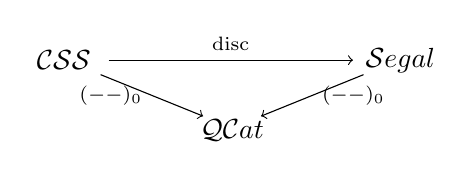
\begin{tikzpicture}[x=1.9em,y=1.5em]
  \node (css)   at (0,1.7)   {$\CSS$};
  \node (segal) at (6.4,1.7) {$\Segal$};
  \node (qcat)  at (3.2,0)   {$\QCat$};
  \draw[->] (0.85,1.7) -- node[above]{$\scriptstyle\rvDisc$} (5.5,1.7);
  \draw[->] (0.7,1.35) -- node[left]{$\scriptstyle(\text{--})_{0}$} (2.65,0.35);
  \draw[->] (5.7,1.35) -- node[right]{$\scriptstyle(\text{--})_{0}$} (3.75,0.35);
\end{tikzpicture}
\end{center}
这最容易通过在模型范畴层面考虑这些函子的\trLeftAdjoint{}而看出。然而，
离散化并不与诸 $\rvNerve$ 构造严格交换，只是在等价意义下交换。对一个%
\trQuasiCategory{} $A$，$\rvNerve(A)$ 是这样一个\trSegalCategories：其
$(m,n)$-单纯形由单纯映射 $\Delta[m]\times\Delta[n]\to A$ 之集给出，这些映射
在 $\Delta[m]$ 的每个顶点处的分量均为常值。相比之下，$\rvDisc(\rvNerve(A))$
是这样一个\trSegalCategories：其 $(m,n)$-单纯形由单纯映射 $\Delta[m]\times\qcInt[n]\to A$ 之集给出，这些映射在 $\Delta[m]$ 的每个顶点处的分量均为
常值。
\end{remark}

从附录 D 中的\cref{dig:saturation-higher-simplices}回忆起：一个 $1$-复状%
\trSimplicialSet{}是一个 $1$-平凡且饱和的复状\trSimplicialSet（见附录 D 中的
\cref{def:complicial-set}、\cref{def:n-trivial}与\cref{def:1-saturated}）。
附录 D 中的\cref{thm:natural-marking-complicial}把诸\trQuasiCategory{}与
$1$-复状\trSimplicialSet——它们在那里被称作「自然标记拟范畴」——等同起来，
因此毫不意外：

\begin{proposition}\label{prop:one-complicial-cosmos}
$1$-复状\trSimplicialSet{}的全子范畴 $\OneComp\hookrightarrow1\text{-}\sSet^{+}$ 定义一个\trCartesianClosed{}\trInfinityCosmos，其中%
\trFunctorSpace{} $\Fun(A,B)$ 定义为\trInternalHom{} $B^{A}$ 的底%
\trQuasiCategory。相对于这一\trInfinityCosmos{}结构，底\trQuasiCategory{}%
\trFunctor{} $(\text{--})_{0}\colon\OneComp\rightleftarrows\QCat$ 与自然标记%
\trFunctor{} $(\text{--})^{\natural}\colon\QCat\rightleftarrows\OneComp$ 都是%
\trCosmological。
\end{proposition}
\begin{proof}
由 Lurie \cite[\S3.1.3--4]{bib78} 与 Verity \cite[\S6.5]{bib129} 各自独立的
定理，诸自然标记拟范畴——我们称之为\textbf{$1$-复状\trSimplicialSet}——
构成承载于\trMarkedSimplicialSet{}的\trCategory{}之上的一个%
\trCartesianClosed{}\trModelStructure{}的诸\trFibrant{}对象，其中一切对象
皆\trCofibrant。存在一个伴随
\begin{center}
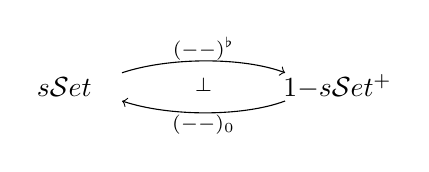
\begin{tikzpicture}[x=1.9em,y=1.5em]
  \node (s) at (0,0)   {$\sSet$};
  \node (c) at (5.2,0) {$1\text{-}\sSet^{+}$};
  \draw[->] (1.1,0.34) .. controls (2.0,0.72) and (3.4,0.72) .. (4.2,0.34);
  \node at (2.65,0.92) {$\scriptstyle(\text{--})^{\flat}$};
  \node at (2.65,0.05) {$\scriptstyle\bot$};
  \draw[->] (4.2,-0.34) .. controls (3.4,-0.72) and (2.0,-0.72) .. (1.1,-0.34);
  \node at (2.65,-0.92) {$\scriptstyle(\text{--})_{0}$};
\end{tikzpicture}
\end{center}
其中\trRightAdjoint{}遗忘标记，而\trLeftAdjoint{}给每个单纯集指派极小
$1$-平凡标记；Lurie 证明了后者是拟范畴模型结构与 $1$-复状\trSimplicialSet{}%
模型结构之间的一个 Quillen \trEquivalence{} \cite[3.1.5.1]{bib78}。经检视，
其\trLeftAdjoint{}保持有限\trProduct，\footnote{注意，作为带标记单纯集，
$(\Delta[1]\times\Delta[1])^{\flat}\ne\Delta[1]^{\flat}\times\Delta[1]^{\flat}$；
因此，有限积保持性质要想成立，极小标记函子落入 $1$-平凡带标记单纯集的%
\trCategory{}之中是本质性的。}于是\cref{cor:cartesian-closed-cosmos}适用，
从而在全子范畴 $\OneComp$ 上创造一个\trCartesianClosed{}\trInfinityCosmos{}结构，使得\trForgetfulFunctor{}定义一个%
\trCosmologicalBiequivalence{} $(\text{--})_{0}\colon\OneComp\rightleftarrows\QCat$，它与底\trQuasiCategory{}\trFunctor{}重合。$1$-复状\trSimplicialSet{}%
的\trModelCategory{}经由此构造而富集于拟范畴模型结构之上，这一事实已在
\cite[3.1.4.5]{bib78} 中被观察到。

对任何拟范畴 $A$ 与 $B$，观察到存在一个自然\trIsomorphism{}
$\Fun(A,B)\cong\Fun(A^{\natural},B^{\natural})$：一侧是 $\QCat$ 中的函子%
\trQuasiCategory，另一侧是刚刚定义的、$\OneComp$ 中介于其自然标记之间的%
\trFunctorSpace；要点在于，单纯映射 $A\to B$ 保持诸\trIsomorphism，从而保持
自然标记。Verity 证明：自然标记函子 $(\text{--})^{\natural}\colon\QCat\to\OneComp$ 创造诸\trFibrant{}对象之间的诸\trFibration{} \cite[114--118]{bib129}。
由于 $\QCat$ 与 $\OneComp$ 中的诸\trLimit{}都在 $s\Set$ 中被创造，由此得出：
函子 $(\text{--})^{\natural}\colon\QCat\to\OneComp$ 是一个%
\trCosmologicalBiequivalence，而且确是 $(\text{--})_{0}\colon\OneComp\to\QCat$
的一个逆\trIsomorphism。
\end{proof}

\subsection*{练习}

\begin{exercise}\label{ex:pcat-presheaves-quotient}
Joyal 与 Tierney 把子范畴 $\PCat\hookrightarrow\Set^{\Delta^{\mathrm{op}}\times\Delta^{\mathrm{op}}}$ 等同于由 $\Delta\times\Delta$ 的 $1$-范畴性商
$\Delta\vert_{2}$ 所索引的预层\trCategory，这一商由逆转函子
$[0]\times\Delta\hookrightarrow\Delta\times\Delta$ 像中的诸映射而定义
\cite[5.4]{bib64}。从这一观点出发，重新定义\cref{prop:segal-cosmos}之证明中
出现的、介于 $\PCat$、$\Set^{\Delta^{\mathrm{op}}\times\Delta^{\mathrm{op}}}$
与 $\Set^{\Delta^{\mathrm{op}}}$ 之间的三个伴随。
\end{exercise}

\begin{exercise}\label{ex:nerve-sections}
验证：诸\trCosmologicalBiequivalence{} $\rvNerve\colon\QCat\rightleftarrows\CSS$
与 $\rvNerve\colon\QCat\rightleftarrows\Segal$ 各自定义相应底%
\trQuasiCategory{}函子的一个\trSection。
\end{exercise}

   %

\providecommand{\Fun}{\operatorname{Fun}}
\providecommand{\Cat}{\mathcal{C}at}
\providecommand{\sSet}{s\mathcal{S}et}
\providecommand{\Set}{\mathcal{S}et}
\providecommand{\QCat}{\mathcal{Q}\mathcal{C}at}
\providecommand{\ssSet}{ss\mathcal{S}et}%
\providecommand{\CSS}{\mathcal{C}\mathcal{S}\mathcal{S}}
\providecommand{\OneComp}{1\text{-}\mathcal{C}omp}
\providecommand{\qcOne}{\mathbf{1}}   %
\providecommand{\qcInt}{\mathbb{I}}   %
\providecommand{\rvWarrow}{\rightsquigarrow}%

\section{\texorpdfstring{$(\infty,n)$}{(∞,n)}-\trCategory{}的%
\trInfinityCosmos}\label{sec:infinity-cosmoi-of-infinity-n-categories}

在本节中，我们引入各式各样的\trInfinityCosmos，其对象是一些 $(\infty,n)$-%
\trCategory（$1<n\le\oo$）的模型。这些\trInfinityCosmos{}描述了诸%
\trInfinityCategory、诸\trInfinityFunctor{}与诸\trInfinityNaturalTransformation{}%
的 $(\infty,2)$-\trCategory，其间略去更高维的变换；不过，诸\trGeneralizedElement{}%
与诸\trInternalHom{}仍使我们得以触及高维的非可逆态射。

由于完整地规定一个 $(\infty,n)$-\trCategory{}的模型所牵涉的组合学可能相当繁难，
为省篇幅，我们不对这里讨论的每一个高阶范畴论概念都给出定义，而是提供指出这些
定义所在之处的外部引注。

我们的几个 $(\infty,n)$-\trCategory{}模型被定义为经一个 1-\trCategory{}
$\boldsymbol{\Theta}_{n}$ 所索引的预层——该\trCategory{}由 Joyal 在一篇未发表的
札记中最先引入 \cite{bib60}，我们这里呈献的是归于 Berger 的一个等价形式
\cite{bib11}。

\begin{definition}\label{def:theta-categories}
对 $0\le n\le\oo$，归纳地定义一族 1-\trCategory{} $\boldsymbol{\Theta}_{n}$ 如下。
\begin{itemize}
\item $\boldsymbol{\Theta}_{0}\coloneqq\qcOne$ 是\trTerminal{}范畴，而
  $\boldsymbol{\Theta}_{1}\coloneqq\Delta$ 是由有限非空序数与保序映射构成的%
  \trCategory。
\item $\boldsymbol{\Theta}_{n}\coloneqq\Delta\wr\boldsymbol{\Theta}_{n-1}$，其中
  $\Delta\wr\text{--}\colon\Cat\to\Cat$ 是\textbf{\trWreathProduct}（categorial
  wreath product）构造。显式地，对一个 1-\trCategory{} $C$，$\Delta\wr C$
  是这样的\trCategory：
  \begin{itemize}
  \item 其对象是诸二元组 $[n](c_{1},\dots,c_{n})$，其中 $[n]\in\Delta$ 且
    $c_{i}\in C$；
  \item 其态射 $(\alpha;\bar{f})\colon[n](c_{1},\dots,c_{n})\to[m](c'_{1},\dots,c'_{m})$ 由一个单纯映射
    $\alpha\colon[n]\to[m]\in\Delta$
    连同诸态射 $f_{i,j}\colon c_{i}\to c'_{j}\in C$ 给出，后者对一切
    $0<i\le n$ 与 $\alpha(i-1)<j\le\alpha(i)$。
  \end{itemize}
\end{itemize}
\end{definition}

$\boldsymbol{\Theta}_{n}$ 的对象定义 $0\le k\le n$ 时 k-\trCell{}的%
\trPastingDiagram，而其态射定义投影、复合与退化映射。把一个\trPastingDiagram{}%
送到由它生成的自由严格 $n$-\trCategory{}的那个\trFunctor{}
$\boldsymbol{\Theta}_{n}\to n\text{-}\Cat$ 是\trFullyFaithful{}
\cite[3.7]{bib11}。

例如，$\boldsymbol{\Theta}_{2}$ 中的态射
$(\delta^{2};(\delta^{1},!,\mathrm{id}))\colon[2]([1],[1])\to[3]([2],[0],[1])$
对应于由下列\trPastingDiagram{}所生成的自由 2-\trCategory{}之间的一个%
\trTwoFunctor：
\begin{center}
\begin{tikzpicture}[x=1.9em,y=1.3em]
  \node (a0) at (0,0) {$0$};
  \node (a1) at (2.6,0) {$1$};
  \node (a2) at (5.2,0) {$2$};
  \draw[->] (0.45,0.18) -- (2.15,0.18);
  \draw[->] (0.45,-0.18) -- (2.15,-0.18);
  \node at (1.3,0) {$\scriptstyle\Downarrow$};
  \draw[->] (3.05,0.18) -- (4.75,0.18);
  \draw[->] (3.05,-0.18) -- (4.75,-0.18);
  \node at (3.9,0) {$\scriptstyle\Downarrow$};
  \node at (7.1,0) {$\mapsto$};
  \begin{scope}[shift={(8.8,0)}]
    \node (b0) at (0,0) {$0$};
    \node (b1) at (2.6,0) {$1$};
    \node (b2) at (5.2,0) {$2$};
    \node (b3) at (7.8,0) {$3$};
    \draw[->] (0.45,0.18) -- (2.15,0.18);
    \draw[->] (0.45,-0.18) -- (2.15,-0.18);
    \node at (1.3,0.55) {$\scriptstyle\Downarrow$};
    \node at (1.3,-0.55) {$\scriptstyle\Downarrow$};
    \draw[->] (3.05,0) -- (4.75,0);
    \draw[->] (5.65,0.18) -- (7.35,0.18);
    \draw[->] (5.65,-0.18) -- (7.35,-0.18);
    \node at (6.5,0) {$\scriptstyle\Downarrow$};
  \end{scope}
\end{tikzpicture}
\end{center}
它把 0 送到 0、把 1 送到 1、把 2 送到 3，并把定义域的左 2-\trCell{}送到余定义域
最左侧诸 2-\trCell{}的竖直复合，把定义域的右 2-\trCell{}送到余定义域最右侧的
2-\trCell{}与中央 1-\trCell{}的\trWhiskering。

\begin{lemma}\label{lem:wreath-product-adjunction}
对任何带有一个\trTerminal{}元素 $t$ 的 1-\trCategory，下方左侧的\trAdjunction{}%
诱导下方右侧的\trAdjunction：
\begin{center}
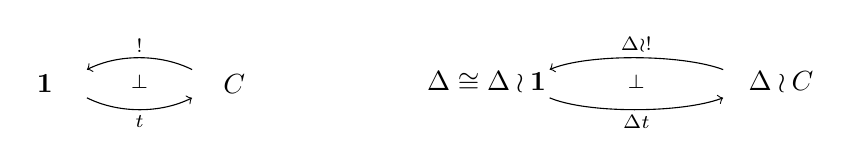
\begin{tikzpicture}[x=1.9em,y=1.5em]
  \node (a) at (0,0) {$\qcOne$};
  \node (b) at (3.6,0) {$C$};
  \draw[->] (2.8,0.34) .. controls (2.2,0.72) and (1.4,0.72) .. (0.8,0.34);
  \node at (1.8,0.92) {$\scriptstyle!$};
  \node at (1.8,0.05) {$\scriptstyle\bot$};
  \draw[->] (0.8,-0.34) .. controls (1.4,-0.72) and (2.2,-0.72) .. (2.8,-0.34);
  \node at (1.8,-0.92) {$\scriptstyle t$};
  \node at (5.7,0) {$\rvWarrow$};
  \begin{scope}[shift={(8.4,0)}]
    \node (c) at (0,0) {$\Delta\cong\Delta\wr\qcOne$};
    \node (d) at (5.6,0) {$\Delta\wr C$};
    \draw[->] (4.5,0.34) .. controls (3.7,0.72) and (1.9,0.72) .. (1.2,0.34);
    \node at (2.85,0.92) {$\scriptstyle\Delta\wr!$};
    \node at (2.85,0.05) {$\scriptstyle\bot$};
    \draw[->] (1.2,-0.34) .. controls (1.9,-0.72) and (3.7,-0.72) .. (4.5,-0.34);
    \node at (2.85,-0.92) {$\scriptstyle\Delta t$};
  \end{scope}
\end{tikzpicture}
\end{center}
\end{lemma}
\begin{proof}
\trWreathProduct{}定义一个 2-\trFunctor{}
$\Delta\wr\text{--}\colon\Cat\to\Cat$。
\end{proof}

Ara 引入了一个对每个 $1\le n<\oo$ 的 $(\infty,n)$-\trCategory{}之模型，称作
\textbf{$n$-拟范畴}（$n$-quasi-categories），即 $\boldsymbol{\Theta}_{n}$ 之上由
一个特别的右\trLifting{}性质所刻画的预层，该性质描述于 \cite[\S5]{bib4}。
Ara 的 1-拟范畴与通常的\trQuasiCategory{}相重合。

\begin{proposition}\label{prop:n-quasi-category-cosmos}
对每个 $n\ge 1$，诸 $n$-拟范畴的全子范畴
$n\text{-}\QCat\hookrightarrow\Set^{\boldsymbol{\Theta}_{n}^{\mathrm{op}}}$
定义一个\trCartesianClosed{}\trInfinityCosmos。
\end{proposition}
\begin{proof}
Ara 在\trCategory{}
$\Set^{\boldsymbol{\Theta}_{n}^{\mathrm{op}}}$ 上构造了一个\trCartesianClosed{}%
\trModelStructure——它在 $n=1$ 的情形推广了 Joyal \trModelStructure——其中诸%
\trFibrant{}对象恰是诸 $n$-拟范畴，而诸余纤维化是诸\trMonomorphism{}
\cite{bib4}；特别地，一切对象皆\trCofibrant。于是，要在全子范畴
$n\text{-}\QCat$ 上诱导一个\trCartesianClosed{}\trInfinityCosmos{}结构，
只须找到一支从这一\trModelStructure{}通往拟范畴之\trModelStructure{}的
Quillen \trAdjunction，使其\trLeftAdjoint{}
$\Set^{\Delta^{\mathrm{op}}}\to\Set^{\boldsymbol{\Theta}_{n}^{\mathrm{op}}}$ 保持
二元\trProduct。

为此，注意到 $[0]\in\boldsymbol{\Theta}_{n-1}$ 对一切 $n>1$ 是\trTerminal{}的，
于是\cref{lem:wreath-product-adjunction}提供了如下方左侧的一个\trAdjunction，
从而也提供了如下方右侧的一个\trAdjunction：
\begin{center}
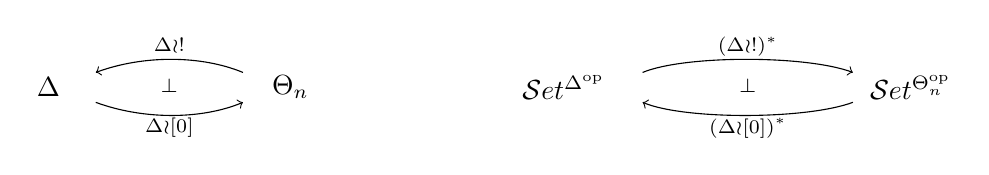
\begin{tikzpicture}[x=1.9em,y=1.5em]
  \node (d) at (0,0) {$\Delta$};
  \node (t) at (4.6,0) {$\boldsymbol{\Theta}_{n}$};
  \draw[->] (3.7,0.36) .. controls (2.9,0.78) and (1.8,0.78) .. (0.9,0.36);
  \node at (2.3,0.98) {$\scriptstyle\Delta\wr!$};
  \node at (2.3,0.05) {$\scriptstyle\bot$};
  \draw[->] (0.9,-0.36) .. controls (1.8,-0.78) and (2.9,-0.78) .. (3.7,-0.36);
  \node at (2.3,-0.98) {$\scriptstyle\Delta\wr[0]$};
  \node at (7.0,0) {$\rvWarrow$};
  \begin{scope}[shift={(9.8,0)}]
    \node (s) at (0,0) {$\Set^{\Delta^{\mathrm{op}}}$};
    \node (p) at (6.6,0) {$\Set^{\boldsymbol{\Theta}_{n}^{\mathrm{op}}}$};
    \draw[->] (1.5,0.36) .. controls (2.3,0.78) and (4.6,0.78) .. (5.5,0.36);
    \node at (3.5,0.98) {$\scriptstyle(\Delta\wr!)^{\ast}$};
    \node at (3.5,0.05) {$\scriptstyle\bot$};
    \draw[->] (5.5,-0.36) .. controls (4.6,-0.78) and (2.3,-0.78) .. (1.5,-0.36);
    \node at (3.5,-0.98) {$\scriptstyle(\Delta\wr[0])^{\ast}$};
  \end{scope}
\end{tikzpicture}
\end{center}
\trRightAdjoint{}
$\Delta\wr[0]\colon\Delta\hookrightarrow\boldsymbol{\Theta}_{n}$ 把 $\Delta$ 包含
为「仅由 1-\trCell{}组成的\trPastingDiagram」之子范畴；于是，沿这一\trFunctor{}%
的限制 $(\Delta\wr[0])^{\ast}\colon\Set^{\boldsymbol{\Theta}_{n}^{\mathrm{op}}}\to\Set^{\Delta^{\mathrm{op}}}$ 忘掉高维胞腔。另一支伴随
$\Delta\wr!\colon\boldsymbol{\Theta}_{n}\to\Delta$ 投影到\trWreathProduct{}的第一分量上。
注意到预层\trCategory{}之间相应的限制\trFunctor{}拥有它自己的一个\trLeftAdjoint%
——由左\trKanExtension{}所定义——从而显然保持诸\trProduct。

的确，出于同一理由，这一\trLeftAdjoint{}保持一切\trLimit，从而也保持诸%
\trMonomorphism（它们可以刻画为其\trKernelPair（kernel pair）由恒同给出的那些映射）。
据 Joyal 与 Tierney 的一个结果 \cite[7.15]{bib64}，要证明一支\trAdjunction{}是
Quillen 的，只须证明其\trLeftAdjoint{}保持诸余纤维化——如我们刚刚所做的——
而其\trRightAdjoint{}保持\trFibrant{}对象之间的诸\trFibration。据
\cref{lem:adjunction-transposes-lifting}，这意味着我们只须验证：这一%
\trLeftAdjoint{}把诸内号角包含
$\{\Lambda^{k}[n]\hookrightarrow\Delta[n]\}_{n\ge2,0<k<n}$ 与映射
$\qcOne\hookrightarrow\qcInt$ 载为 Ara 的\trModelStructure{}中的诸平凡余纤维化。
事实上，由 \cite[3.5]{bib64}，只须考虑诸脊柱包含
$\{\Gamma[n]\hookrightarrow\Delta[n]\}_{n\ge2}$ 以替代诸内号角包含——我们也将
如此行事。

为看到这一点，有益的是注意到——如 \cite[\S6]{bib4} 中所观察——这一%
\trLeftAdjoint{}与严格 1-\trCategory{}和严格 $n$-\trCategory{}的诸神经嵌入相
交换：
\begin{center}
\begin{tikzpicture}[x=1.9em,y=1.5em]
  \node (cat)  at (0,1.4) {$\Cat$};
  \node (ncat) at (5.8,1.4) {$n\text{-}\Cat$};
  \node (setd) at (0,-1.4) {$\Set^{\Delta^{\mathrm{op}}}$};
  \node (sett) at (5.8,-1.4) {$\Set^{\boldsymbol{\Theta}_{n}^{\mathrm{op}}}$};
  \draw[right hook->] (0.95,1.4) -- (4.75,1.4);
  \draw[->] (ncat) -- (sett);
  \draw[right hook->] (cat) -- (setd);
  \draw[->] (1.7,-1.4) -- node[above]{$\scriptstyle(\Delta\wr[0])^{\ast}$} (4.0,-1.4);
\end{tikzpicture}
\end{center}
特别地，这一\trLeftAdjoint{}把 $\qcOne\hookrightarrow\qcInt$ 的 1-范畴性神经
送到这一映射的严格 $n$-范畴性神经；而且，由于这一\trLeftAdjoint{}也保持诸%
\trColimit，它把脊柱包含 $\Gamma[n]\hookrightarrow\Delta[n]$ 送到对象
$[n]([0],\dots,[0])\in\boldsymbol{\Theta}_{n}$ 的相应的「脊柱包含」。由于这两类
映射都属于 Ara 的「$n$-拟范畴的\trLocalizer」（\cite[5.17]{bib4}），它们必定是
平凡余纤维化。于是，这支伴随如所断言是 Quillen 的，而\cref{cor:cartesian-closed-cosmos}%
适用于在 $n\text{-}\QCat$ 上创造一个\trCartesianClosed{}\trInfinityCosmos{}%
结构。
\end{proof}

另一类 $(\infty,n)$-\trCategory{}的模型，对 $0\le n<\oo$，归于 Rezk
\cite{bib101}。一个\textbf{$\boldsymbol{\Theta}_{n}$-空间}（$\boldsymbol{\Theta}_{n}$-space）
是 $\boldsymbol{\Theta}_{n}$ 上的一个单纯预层，满足与\cref{def:complete-segal-space}%
的那些条件相类比的 Reedy 纤维性、Segal 与完全性诸条件。一个
$\boldsymbol{\Theta}_{1}$-空间恰是一个\trCompleteSegalSpaces，而一个
$\boldsymbol{\Theta}_{0}$-空间只不过是一个\trKanComplex。

\begin{proposition}\label{prop:theta-space-cosmos}
对每个 $n\ge 1$，诸 $\boldsymbol{\Theta}_{n}$-空间的全子范畴
$\boldsymbol{\Theta}_{n}\text{-}\mathcal{S}p\hookrightarrow\ssSet^{\boldsymbol{\Theta}_{n}^{\mathrm{op}}}$ 定义一个\trCartesianClosed{}%
\trInfinityCosmos，对其而言，底\trCompleteSegalSpaces{}函子
$U\colon\boldsymbol{\Theta}_{n}\text{-}\mathcal{S}p\to\boldsymbol{\Theta}_{1}\text{-}\mathcal{S}p\cong\CSS$ 是\trCosmological。
\end{proposition}
\begin{proof}
Rezk 在\trCategory{}
$\ssSet^{\boldsymbol{\Theta}_{n}^{\mathrm{op}}}$ 上构造了一个\trCartesianClosed{}%
\trModelStructure，它在 $n=1$ 的情形推广了他的\trCompleteSegalSpaces{}之%
\trModelStructure，其中诸\trFibrant{}对象恰是诸 $\boldsymbol{\Theta}_{n}$-空间，
而诸余纤维化是诸\trMonomorphism{} \cite{bib101}；特别地，一切对象皆%
\trCofibrant。于是，要在全子范畴 $\boldsymbol{\Theta}_{n}\text{-}\mathcal{S}p$ 上
诱导一个\trCartesianClosed{}\trInfinityCosmos{}结构，只须找到一支介于这一%
\trModelStructure{}与\trCompleteSegalSpaces{}之\trModelStructure{}之间的
Quillen \trAdjunction，使其\trLeftAdjoint{}
$\sSet^{\Delta^{\mathrm{op}}}\to\ssSet^{\boldsymbol{\Theta}_{n}^{\mathrm{op}}}$
保持二元\trProduct。随后，我们把这一伴随与伴随 \eqref{eq:pi-iota-adjunction}
的复合施用\cref{cor:cartesian-closed-cosmos}。

一如\cref{prop:n-quasi-category-cosmos}的证明，我们经由把
\cref{lem:wreath-product-adjunction}施用于\trTerminal{}对象
$[0]\in\boldsymbol{\Theta}_{n-1}$ 而得到所需的伴随：
\begin{rveq}\label{eq:theta-space-adjunction}
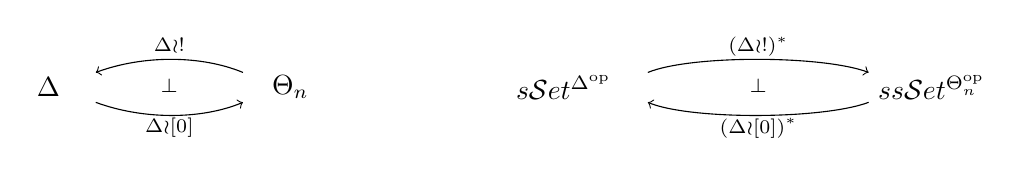
\begin{tikzpicture}[x=1.9em,y=1.5em]
  \node (d) at (0,0) {$\Delta$};
  \node (t) at (4.6,0) {$\boldsymbol{\Theta}_{n}$};
  \draw[->] (3.7,0.36) .. controls (2.9,0.78) and (1.8,0.78) .. (0.9,0.36);
  \node at (2.3,0.98) {$\scriptstyle\Delta\wr!$};
  \node at (2.3,0.05) {$\scriptstyle\bot$};
  \draw[->] (0.9,-0.36) .. controls (1.8,-0.78) and (2.9,-0.78) .. (3.7,-0.36);
  \node at (2.3,-0.98) {$\scriptstyle\Delta\wr[0]$};
  \node at (7.0,0) {$\rvWarrow$};
  \begin{scope}[shift={(9.8,0)}]
    \node (s) at (0,0) {$\sSet^{\Delta^{\mathrm{op}}}$};
    \node (p) at (7.0,0) {$\ssSet^{\boldsymbol{\Theta}_{n}^{\mathrm{op}}}$};
    \draw[->] (1.6,0.36) .. controls (2.4,0.78) and (4.9,0.78) .. (5.8,0.36);
    \node at (3.7,0.98) {$\scriptstyle(\Delta\wr!)^{\ast}$};
    \node at (3.7,0.05) {$\scriptstyle\bot$};
    \draw[->] (5.8,-0.36) .. controls (4.9,-0.78) and (2.4,-0.78) .. (1.6,-0.36);
    \node at (3.7,-0.98) {$\scriptstyle(\Delta\wr[0])^{\ast}$};
  \end{scope}
\end{tikzpicture}
\end{rveq}
其\trLeftAdjoint{}拥有一个更进一层的\trLeftAdjoint——由左\trKanExtension{}所
给出——从而保持诸\trProduct。

尚须论证的只是这支伴随是 Quillen 的。$\boldsymbol{\Theta}_{n}$-空间之%
\trModelStructure——并且，经特化，\trCompleteSegalSpaces{}之%
\trModelStructure——被定义为单纯预层上内射（或者等价地，Reedy）%
\trModelStructure{}的一个\trBousfieldLocalization。在\trInjectiveModelStructure{}中，
诸余纤维化与诸平凡余纤维化在 $\sSet$ 中逐点定义，故这一\trLeftAdjoint{}相对
于这些\trModelStructure{}显然是左 Quillen 的。于是，这支伴随对局部化后的诸%
\trModelStructure{}是 Quillen 的，当且仅当其\trRightAdjoint{}——即 Rezk 称作
「底单纯空间」的那个\trFunctor——保持诸\trFibrant{}对象；因为在此情形，这一%
\trLeftAdjoint{}保持新的诸平凡余纤维化，而后者正是由前者来定义的。一个函子
$X\in\ssSet^{\boldsymbol{\Theta}_{n}^{\mathrm{op}}}$ 是\trFibrant{}的，当且仅当它
满足 Reedy、Segal 与完全性诸条件。由于伴随 \eqref{eq:theta-space-adjunction}
对内射/Reedy \trModelStructure{}是 Quillen 的，Reedy 纤维性条件得以保持，而
Rezk 证明了 Segal 条件也得以保持 \cite[7.2]{bib101}。诸 $\boldsymbol{\Theta}_{n}$%
-空间的完全性条件由底单纯空间的完全性条件所创造 \cite[\S7]{bib101}，故这一
条件同样得以保持。于是，\trRightAdjoint{} \eqref{eq:theta-space-adjunction}
限制为一个函子 $U\colon\boldsymbol{\Theta}_{n}\text{-}\mathcal{S}p\to\CSS$，我们
称之为\textbf{底\trCompleteSegalSpaces{}函子}（underlying complete Segal
space functor）。

\cref{cor:cartesian-closed-cosmos}适用于在
$\boldsymbol{\Theta}_{n}\text{-}\mathcal{S}p$ 上创造一个\trCartesianClosed{}%
\trInfinityCosmos{}结构。由\cref{lem:finite-product-adjunction-v-enriched}，
伴随 \eqref{eq:theta-space-adjunction} 富集于双单纯集之上，于是
\cref{prop:change-of-base-model-cosmoi}可用来证明底\trCompleteSegalSpaces{}%
函子是\trCosmological。
\end{proof}

还存在另一个 $(\infty,n)$-\trCategory{}的模型，它推广了 $(\infty,1)$-%
\trCategory{}的\trCompleteSegalSpaces{}模型，并利用了取值于一个\trModelCategory{}%
中的\textbf{\trRezkObject}（Rezk object）这一概念：

\begin{definition}\label{def:rezk-objects}
设 $\mathcal{M}$ 是一个\trModelCategory。
\begin{enumerate}[label=(\roman*)]
\item 一个\trSimplicialObject{}
  $X_{\bullet}\in\mathcal{M}^{\Delta^{\mathrm{op}}}$ 是\textbf{Reedy 纤维性}的，
  恰当其在诸\trWeightedLimit{}上诱导的映射
  \[
  X_{m}\cong\operatorname{lim}_{\Delta[m]}X\longrightarrow
  \operatorname{lim}_{\partial\Delta[m]}X=:\ M_{m}X
  \]
  对一切 $m\ge 0$ 都是一个\trFibration。
\item 一个 Reedy 纤维性的\trSimplicialObject{} $X_{\bullet}$ 是一个%
  \textbf{\trSegalObject}（Segal object），恰当其在诸\trWeightedLimit{}上诱导的
  映射
  \[
  X_{n}\cong\operatorname{lim}_{\Delta[n]}X\longrightarrow
  \operatorname{lim}_{\Lambda^{k}[n]}X
  \]
  对一切 $n\ge 2$ 与 $0<k<n$ 都是一个\trTrivialFibration。
\item 一个\trSegalObject{} $X_{\bullet}$ 是一个\textbf{\trRezkObject}，恰当其在诸%
  \trWeightedLimit{}上诱导的映射
  \[
  \operatorname{lim}_{\qcInt}X\longrightarrow
  \operatorname{lim}_{\Delta[0]}X\cong X_{0}
  \]
  是一个\trTrivialFibration。
\end{enumerate}
\end{definition}

一个映射 $p\colon X_{\bullet}\to Y_{\bullet}\in\mathcal{M}^{\Delta^{\mathrm{op}}}$
是一个\textbf{\trRezkIsofibration}（Rezk isofibration），若出现于 (i)、(ii) 与
(iii) 中的那些映射的相对类比——它们由 $p$ 与相应的诸权之映射所作的 Leibniz
加权\trWeightedLimit{}而形成——分别是\trFibration、\trTrivialFibration{}与一个%
\trTrivialFibration。

我们对\cref{def:complete-segal-space}的表述与 Rezk 对其诸条件的原有框架略有
出入，其意在使人看清：诸\trCompleteSegalSpaces{}恰好是取值于 Quillen 的%
\trKanComplex{}之\trModelStructure{}中的诸\trRezkObject。

\begin{proposition}\label{prop:rezk-cosmos}
试设 $\mathcal{M}$ 是一个 \emph{\trCisinskiModelCategory}。\footnote{一个%
\textbf{\trCisinskiModelStructure}（Cisinski model structure）是一个%
\trGrothendieckTopos（Grothendieck topos）上的组合模型结构，其中诸余纤维化恰是诸%
\trMonomorphism。由此可得：$\mathcal{M}^{\Delta^{\mathrm{op}}}$ 上的 Reedy
\trModelStructure{}与\trInjectiveModelStructure{}相重合，并且特别地，一切对象皆%
\trCofibrant{} \cite{bib27,bib16}。}于是，诸\trRezkObject{}的全子范畴
$\mathcal{R}ezk_{\mathcal{M}}\hookrightarrow\mathcal{M}^{\Delta^{\mathrm{op}}}$
定义一个\trInfinityCosmos。
\end{proposition}
\begin{proof}
我们直接从\cref{prop:fibrant-objects-cosmos}出发证明这一结果，办法是证明：
$\mathcal{M}^{\Delta^{\mathrm{op}}}$ 上 Reedy \trModelStructure{}的一个%
\trBousfieldLocalization{}定义一个\trCisinskiModelStructure，它富集于拟范畴之%
\trModelStructure{}之上，而其\trFibrant{}对象恰是诸\trRezkObject。

首先，观察到\trCategory{}
$\mathcal{M}^{\Delta^{\mathrm{op}}}$ 是单纯富集、单纯张量且单纯余张量的，其
hom-空间被富于暗示地记作「$\Fun$」：
\[
(\otimes,\{,\},\Fun)\colon\sSet\times\mathcal{M}^{\Delta^{\mathrm{op}}}
\to\mathcal{M}^{\Delta^{\mathrm{op}}}
\]
并且使得单纯集的诸\trMonomorphism{}与（平凡的）Reedy 余纤维化的 Leibniz
张量是（平凡的）Reedy 余纤维化 \cite[4.4]{bib35}。我们施用 Jeff Smith 定理
\cite{bib8} 证明 $\mathcal{M}^{\Delta^{\mathrm{op}}}$ 容有一个模型结构，其中：
\begin{itemize}
\item 诸余纤维化是诸\trMonomorphism；
\item 诸\trFibrant{}对象是诸\trRezkObject；
\item \trFibrant{}对象之间的诸\trFibration{}是诸\trRezkIsofibration；并且
\item 诸\trWeakEquivalence{}是诸 \textbf{\trRezkWeakEquivalence}（Rezk weak
  equivalences），即那些对一切\trRezkObject{} $X$ 都诱导\trQuasiCategory{}的一个%
  \trEquivalence{} $w^{\ast}\colon\Fun(V,X)\to\Fun(U,X)$ 的映射
  $w\colon U\to V$。
\end{itemize}

注意到，由伴随，一个映射 $p\colon X\to Y\in\mathcal{M}^{\Delta^{\mathrm{op}}}$
是一个\trRezkIsofibration，当且仅当对 $\mathcal{M}$ 中的一切\trMonomorphism{}
$m\colon A\to B$，单纯集之诱导映射
\[
\Fun(B,X)\xrightarrow{\ \widehat{\Fun}(m,p)\ }
\Fun(A,X)\times_{\Fun(A,Y)}\Fun(B,Y)
\]
是\trQuasiCategory{}之间的一个\trIsofibration。据\cref{cor:leibniz-anodyne}与%
\cref{prop:leibniz-stability-isofibrations}，这成立当且仅当该映射对集合
$I\mathbin{\widehat{\times}}J$ 中的映射具有右\trLifting{}性质，其中
\[
I\coloneqq\{\partial\Delta[n]\hookrightarrow\Delta[n]\}_{n\ge0}
\qquad\text{以及}\qquad
J\coloneqq\{\Lambda^{k}[n]\hookrightarrow\Delta[n]\}_{n\ge2,0<k<n}
\cup\{\qcOne\hookrightarrow\qcInt\}.
\]

再次由伴随，以及\cref{prop:leibniz-construction-preserves}(i)，$p$ 是一个%
\trRezkIsofibration，当且仅当它对诸映射之集
$(i\mathbin{\widehat{\times}}j)_{\ast}m\cong j\mathbin{\widehat{\times}}(i_{\ast}m)$——其中 $i\in I$、$j\in J$，而 $m$
取遍 $\mathcal{M}$ 中的生成余纤维化——具有右\trLifting{}性质，这里 $\ast$
表示点态张量 $\ast\colon\sSet\times\mathcal{M}\to\mathcal{M}^{\Delta^{\mathrm{op}}}$。由于据\cref{prop:reedy-cellularly-generated}，
$\mathcal{M}^{\Delta^{\mathrm{op}}}$ 中的诸 Reedy 余纤维化由诸映射 $i_{\ast}m$
（$i\in I$，而 $m$ 取遍 $\mathcal{M}$ 中的生成余纤维化）之集所胞腔式生成，我们
由伴随得出结论：$p$ 是\trRezkObject{}之间的一个\trRezkIsofibration，当且仅当
\[
\Fun(V,X)\xrightarrow{\ \widehat{\Fun}(c,p)\ }
\Fun(U,X)\times_{\Fun(U,Y)}\Fun(V,Y)
\]
对 $\mathcal{M}^{\Delta^{\mathrm{op}}}$ 中的一切\trMonomorphism{}
$c\colon U\to V$ 都是\trIsofibration。

现在容易验证 Jeff Smith 定理的诸条件。诸\trRezkWeakEquivalence{}是\trAccessible{}且满足%
\trTwoOfThreeProperty。我们论证：诸\trRezkWeakEquivalence{}包含一切 Reedy 弱等价，从而
包含诸 Reedy 平凡纤维化——后者由对诸\trMonomorphism{}的右\trLifting{}性质所
刻画。转置 \cite[4.4]{bib35} 中已就 $\mathcal{M}^{\Delta^{\mathrm{op}}}$ 上的
Reedy \trModelStructure{}所作的诸观察，我们看到：对任何 Reedy 平凡余纤维化
$w\colon U\to V$ 与\trRezkObject{} $X$，$w^{\ast}\colon\Fun(V,X)\to\Fun(U,X)$ 是%
\trQuasiCategory{}之间的一个\trEquivalence。据 Ken Brown \cref{lem:ken-brown}，
当 $w$ 只是一个 Reedy 弱等价时亦然。注意到，一个映射 $w\colon U\to V$ 既是%
\trRezkWeakEquivalence{}又是余纤维化，恰当 $w^{\ast}\colon\Fun(V,X)\to\Fun(U,X)$ 是%
\trQuasiCategory{}之间的一个\trTrivialFibration。这一刻画证明了：诸%
\trRezkWeakEquivalence{}与诸余纤维化组成的类对推出与超限复合封闭。Jeff Smith 定理由此蕴含：
诸\trRezkObject{}的模型结构存在。

要看到\trRezkObject{}的模型结构富集于拟范畴之\trModelStructure{}之上，我们必须
验证
\[
(\otimes,\{,\},\Fun)\colon\sSet\times\mathcal{M}^{\Delta^{\mathrm{op}}}
\to\mathcal{M}^{\Delta^{\mathrm{op}}}
\]
定义一个 Quillen 双变量\trAdjunction（见\cref{def:quillen-two-variable-adjunction}）。
局部化后的\trRezkObject{}之\trModelStructure{}中的诸余纤维化与 $\mathcal{M}^{\Delta^{\mathrm{op}}}$
上 Reedy \trModelStructure{}的诸余纤维化相同，故我们已然知道：诸余纤维化的
Leibniz 张量是余纤维化。为验证这一公理的其余 2/3，我们援引 Dugger 的一个结果
\cite[3.2]{bib35}，它告诉我们：在头一个 1/3 在场的情形下，要验证单纯集的诸%
\trMonomorphism{}与诸平凡余纤维化之 Leibniz 张量是平凡余纤维化，只须证明单纯
余张量 $(\text{--})^{K}\colon\mathcal{M}^{\Delta^{\mathrm{op}}}\to\mathcal{M}^{\Delta^{\mathrm{op}}}$
保持纤维性对象之间的诸\trFibration。对于\trBousfieldLocalization，\trRezkObject{}之间的%
\trRezkIsofibration{}与\trRezkObject{}之间的 Reedy \trFibration{}相重合%
\cite[3.3.16]{bib55}。经直接验证易知 $(\text{--})^{K}$ 保持\trRezkObject，而
Reedy 纤维化之保持则是我们已知的事实之一。

对于 Quillen 双变量\trAdjunction{}的最后 1/3，我们使用 Dugger 结果的第二部分
\cite[3.2]{bib35}，它告诉我们：在前 2/3 在场的情形下，只须验证：对一切%
\trRezkObject{} $Z$ 与单纯集的平凡余纤维化 $j\colon J\to K$，映射
$Z^{j}\colon Z^{K}\to Z^{J}$ 是一个\trRezkWeakEquivalence（这里须假设
$\mathcal{M}^{\Delta^{\mathrm{op}}}$ 是左固有的，而此处情形正是如此，因为一切
对象皆\trCofibrant）。事实上，我们可以证明这一映射是一个\trTrivialFibration：
检验它对诸\trMonomorphism{} $c\colon U\to V\in\mathcal{M}^{\Delta^{\mathrm{op}}}$
的右\trLifting{}性质即可。经转置我们看到：$c$ 对 $Z^{j}$ 可提升，当且仅当 $j$
对 $c^{\ast}\colon\Fun(V,Z)\to\Fun(U,Z)$ 可提升。但我们已验证 $c^{\ast}$ 是%
\trQuasiCategory{}之间的一个\trIsofibration，故所需的提升性质成立。

$\mathcal{M}^{\Delta^{\mathrm{op}}}$ 上\trRezkObject{}的模型结构仍是一个%
\trCisinskiModelStructure，故此构造可以迭代。Barwick 的 \textbf{\trNFoldCompleteSegalSpace}
（$n$-fold complete Segal space）$(\infty,n)$-\trCategory{}模型，经由把%
\trRezkObject{}构造迭代 $n$ 次而形成 \cite{bib6}。将\cref{prop:rezk-cosmos}特化，我们
得出结论：对一切 $n\ge 1$，存在\trNFoldCompleteSegalSpace{}的%
\trInfinityCosmos{} $\CSS_{n}$。
\end{proof}

\begin{remark}\label{rem:rezk-left-proper}
若 $\mathcal{M}$ 是一个左固有组合模型范畴，则刚才给出的证明在
$\mathcal{M}^{\Delta^{\mathrm{op}}}$ 上构造了一个其\trFibrant{}对象为诸%
\trRezkObject{}的\trModelStructure，后者作为一个模型范畴富集于拟范畴之\trModelStructure{}%
之上。唯一的麻烦是：一旦没有 Cisinski 条件，就有可能并非一切\trFibrant{}对象
皆\trCofibrant。尽管如此，这一推广仍可理解为在 \cite[\S2]{bib110} 中所发展的
较弱意义下定义了一个\trInfinityCosmos。
\end{remark}

Verity 在带标记\trSimplicialSet{}的\trCategory{}上构造了一族一般的笛卡尔模型
结构，其\trFibrant{}对象是各种风味的复状单纯集，而其诸\trFibration{}是相应
各种意义的复状等价纤维化 \cite[\S9.3]{bib129}。这些模型结构之一呈现
\cref{prop:one-complicial-cosmos}的\trInfinityCosmos。这里，我们考虑其%
\trFibrant{}对象被称作 \emph{$n$-复状\trSimplicialSet}的模型结构，它们对
$0\le n\le\oo$ 给出 $(\infty,n)$-\trCategory{}的模型；其中「∞-复状单纯集」
是\cref{def:complicial-set}的、在\cref{dig:saturation-higher-simplices}所暗示
并将在证明中详加阐发的那种意义下饱和的复状单纯集。诸定义被安排得使一个
0-复状单纯集是一个（极大标记的）%
\trKanComplex，一个 1-复状单纯集是一个（自然标记的）\trQuasiCategory，而每当
$m<n$ 时，一个 $m$-复状单纯集也是一个 $n$-复状单纯集。

\begin{proposition}\label{prop:n-complicial-cosmos}
对每个 $0\le n\le\oo$，$n$-复状单纯集的\trCategory{}定义一个\trCartesianClosed{}%
\trInfinityCosmos{} $n\text{-}\mathcal{C}omp$。此外，每当 $m<n$，把维数
$k>m$ 的非带标记单纯形全部丢弃的\trFunctor{}
$\mathrm{core}\colon n\text{-}\mathcal{C}omp\to m\text{-}\mathcal{C}omp$
是\trCosmological。
\end{proposition}
\begin{proof}
对于一个由\trMonomorphism{}组成的适当类 $J$，Verity 定义了带标记%
\trSimplicialSet{}的\trCategory{}上的一个\trCartesianClosed{}%
\trModelStructure，其\trFibrant{}对象与其间的诸\trFibration{}是诸 $J$-复状
单纯集与诸 $J$-复状等价纤维化，由对 $J$ 的一个右\trLifting{}性质所刻画
\cite[\S9.3]{bib129}。诸余纤维化是诸\trMonomorphism，故特别地一切对象皆%
\trCofibrant。更详细地说，对诸 $n$-复状单纯集而言，\trMonomorphism{}之类被
定义为
\begin{gather*}
J_{n}\coloneqq\{\Lambda^{k}[m]\hookrightarrow_{r}\Delta^{k}[m]\}_{m\ge1,k\in[m]}
\cup\{\Delta^{k}[m]'\hookrightarrow_{e}\Delta^{k}[m]''\}_{m\ge2,k\in[m]}
\cup{}\\
\{\Delta[r]\hookrightarrow_{e}\Delta[r]_{t}\}_{r>n}\cup
\{\Delta[j]\star\Delta[3]_{\mathrm{eq}}\star\Delta[k]\hookrightarrow
\Delta[j]\star\Delta[3]^{\sharp}\star\Delta[k]\}_{j,k\ge-1}
\end{gather*}
第一族映射是诸复状号角扩张 \eqref{eq:complicial-horn-extension}，而第二族
定义诸复状薄性扩张 \eqref{eq:complicial-thinness-extension}。第三族强加了
「维数大于 $n$ 的一切单纯形皆被标记」这一条件（见\cref{not:marked-simplex-category}），
而最后一个条件是\textbf{饱和}，在其他条件的在场下，它蕴含一切\trEquivalence{}%
皆被标记（见\cref{ex:two-of-six-simplex}与 \cite{bib105}）。为施用 Verity
定理，诸集合 $J_{n}$ 必须满足一些技术性条件，它们在 \cite[91--92]{bib129}
中被列出，并已由 Ozornova 与 Rovelli 就此情形核实 \cite[1.26]{bib89}。由构造，
诸 $n$-复状单纯集栖居于 $n$-平凡带标记\trSimplicialSet{}的子范畴
$n\text{-}\sSet^{+}$ 之中——其中维数大于 $n$ 的一切单纯形皆被标记——而我们
可以把诸\trCartesianClosed{}模型结构限制到这些子范畴上。

诸\trInfinityCosmos{} $0\text{-}\mathcal{C}omp$ 与 $\OneComp$ 分别同构于%
\trInfinityCosmos{} $\mathcal{K}an$ 与 $\QCat$，故我们暂且考虑
$2\le n\le\oo$。为定义\trInfinityCosmos{} $n\text{-}\mathcal{C}omp$，我们
施用\cref{prop:change-of-base-model-cosmoi}，经由一列其\trLeftAdjoint{}保持
二元积的 Quillen 伴随，把这些自富集转换为对\trQuasiCategory{}的富集：
\begin{center}
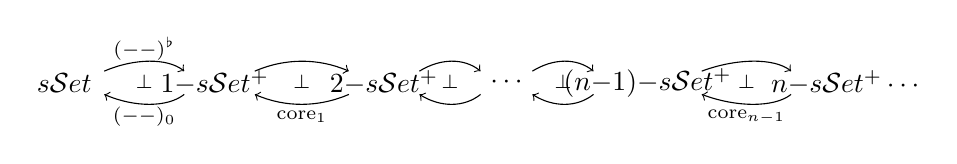
\begin{tikzpicture}[x=1.7em,y=1.4em]
  \node (s) at (0,0)    {$\sSet$};
  \node (a) at (3.2,0)  {$1\text{-}\sSet^{+}$};
  \node (b) at (6.8,0)  {$2\text{-}\sSet^{+}$};
  \node (d) at (9.4,0)  {$\cdots$};
  \node (c) at (12.4,0) {$(n{-}1)\text{-}\sSet^{+}$};
  \node (e) at (16.6,0) {$n\text{-}\sSet^{+}\cdots$};
  \draw[->] (0.85,0.3) .. controls (1.5,0.64) and (2.2,0.64) .. (2.55,0.3);
  \node at (1.7,0.88) {$\scriptstyle(\text{--})^{\flat}$};
  \node at (1.7,0.02) {$\scriptstyle\bot$};
  \draw[->] (2.55,-0.3) .. controls (2.2,-0.64) and (1.5,-0.64) .. (0.85,-0.3);
  \node at (1.7,-0.88) {$\scriptstyle(\text{--})_{0}$};
  \draw[->] (4.05,0.3) .. controls (4.7,0.64) and (5.4,0.64) .. (6.05,0.3);
  \node at (5.05,0.02) {$\scriptstyle\bot$};
  \draw[->] (6.05,-0.3) .. controls (5.4,-0.64) and (4.7,-0.64) .. (4.05,-0.3);
  \node at (5.05,-0.88) {$\scriptstyle\mathrm{core}_{1}$};
  \draw[->] (7.55,0.3) .. controls (8.0,0.64) and (8.5,0.64) .. (8.85,0.3);
  \node at (8.2,0.02) {$\scriptstyle\bot$};
  \draw[->] (8.85,-0.3) .. controls (8.5,-0.64) and (8.0,-0.64) .. (7.55,-0.3);
  \draw[->] (9.95,0.3) .. controls (10.4,0.64) and (10.9,0.64) .. (11.25,0.3);
  \node at (10.6,0.02) {$\scriptstyle\bot$};
  \draw[->] (11.25,-0.3) .. controls (10.9,-0.64) and (10.4,-0.64) .. (9.95,-0.3);
  \draw[->] (13.55,0.3) .. controls (14.3,0.64) and (15.1,0.64) .. (15.45,0.3);
  \node at (14.5,0.02) {$\scriptstyle\bot$};
  \draw[->] (15.45,-0.3) .. controls (15.1,-0.64) and (14.3,-0.64) .. (13.55,-0.3);
  \node at (14.5,-0.88) {$\scriptstyle\mathrm{core}_{n-1}$};
\end{tikzpicture}
\end{center}

在极限情形，我们还考虑伴随
\begin{center}
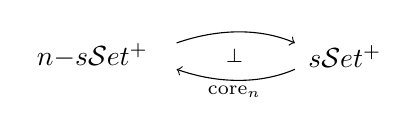
\begin{tikzpicture}[x=1.9em,y=1.4em]
  \node (n) at (0,0) {$n\text{-}\sSet^{+}$};
  \node (s) at (4.8,0) {$\sSet^{+}$};
  \draw[->] (1.6,0.34) .. controls (2.4,0.72) and (3.2,0.72) .. (3.85,0.34);
  \node at (2.7,0.02) {$\scriptstyle\bot$};
  \draw[->] (3.85,-0.34) .. controls (3.2,-0.72) and (2.4,-0.72) .. (1.6,-0.34);
  \node at (2.7,-0.92) {$\scriptstyle\mathrm{core}_{n}$};
\end{tikzpicture}
\end{center}
其中 $\mathrm{core}_{n}X\hookrightarrow X$ 是只包含那些「其维数大于 $n$ 的
诸面皆被标记」的单纯形的单纯子集。由伴随，这些\trFunctor{}把
$(n{+}1)$-复状单纯集载为 $n$-复状单纯集（见\cref{ex:n-core-complicial}）。
由于诸\trLeftAdjoint{}保持诸\trMonomorphism{}与诸\trProduct，这足以验证这些
伴随是 Quillen 的。\cref{cor:cartesian-closed-cosmos}现在诱导出所需的诸%
\trInfinityCosmos，而\cref{cor:right-quillen-adjunction-biequivalence}提供了
诸\trCosmological{}核函子。
\end{proof}

基于 Hirschowitz–Simpson \cite{bib56} 与 Pellissier \cite{bib90} 的既往工作，
Simpson 把\trSegalCategories{}之\trModelStructure{}的构造加以迭代
\cite[\S19.2-4]{bib116}。当基模型范畴取为 Quillen 的\trKanComplex{}之%
\trModelStructure{}时，第 $n$ 次迭代定义了诸 \textbf{Segal $n$-\trCategory}
（Segal $n$-categories），尽管 Simpson 也考虑了更一般的模型范畴论基。在适当
的假设之下——Segal $n$-范畴的情形正满足它们——如此产生的\trModelStructure{}%
是\trCartesianClosed{}且一切对象皆\trCofibrant，这强烈暗示：存在一座由其%
\trFibrant{}对象所张成的\trInfinityCosmos，即诸 Reedy 纤维性的 Segal
$n$-\trCategory。我们把对这一点的确证留给有兴趣的读者作为练习。

\subsection*{练习}

\begin{exercise}\label{ex:rezk-isofibration-formulation}
给出\cref{def:rezk-objects}中用于定义\trRezkIsofibration{}概念的诸条件 (i)、(ii)
与 (iii) 的「相对类比」的一个显式表述。
\end{exercise}

\begin{exercise}\label{ex:segal-n-category-cosmos}
探究 Hirschowitz 与 Simpson 的诸 Segal $n$-\trCategory{} \cite{bib56} 之上的
潜在\trInfinityCosmos{}结构。
\end{exercise}

\begin{exercise}\label{ex:cosmological-biequivalence-search}
搜寻本节所构造的诸\trInfinityCosmos{}之间的诸\trCosmologicalBiequivalence
（并请把你的发现与作者分享）。
\end{exercise}

   %
